\documentclass[22pt, UTF8]{article}
\usepackage{ctex}
\usepackage{graphicx}
\usepackage{multirow}
\usepackage{array}
\usepackage[T1]{fontenc}
\usepackage{mathptmx}
\usepackage{caption}
\usepackage{amsmath, amssymb}
\usepackage{geometry}
\usepackage{fancyhdr}
\usepackage{float}
\usepackage{textcomp}

\geometry{left=3.3cm, right=3.3cm, bottom=3.5cm}
%----------------------------------------------------------------
% 设置页眉和页脚
\pagestyle{fancy}
\lhead{\leftmark} % 页眉的左边显示Section
\rhead{} % 页眉的右边不显示
\renewcommand\headrulewidth{.5pt} % 设置页眉下面的线宽度
\renewcommand\footrulewidth{0pt} % 设置页码上面的线宽度
%-----------------------------------------------------------------
% 设置图片名称的显示格式
\numberwithin{figure}{section}
\captionsetup[figure]{labelfont={bf}, name={Fig.}, labelsep=period}
% 设置表格名称的显示格式
\numberwithin{table}{section}
\captionsetup[table]{labelfont={bf}, name={Tab.}, labelsep=period}
%---------------------------------------------------------------
\numberwithin{equation}{section} % 设置公式序号的显示格式

\makeatletter
\@addtoreset{equation}{section}
\makeatother
%---------------------------------------------------------------
\newcommand{\enabstractname}{Abstract} % 设置摘要的显示格式
\newenvironment{enabstract}{
    \par \fontsize{18pt}{0} % “18”是字符串“Abstract”的大小
    \noindent\mbox{}\hfill{\bfseries \enabstractname}\hfill\mbox{}\par
    \vskip 2.5ex}

\linespread{1.5}

\begin{document}
    
\thispagestyle{empty} % 此页不显示页眉、页码等格式
\begin{center}
    \begin{figure}[H]
        \begin{center}
            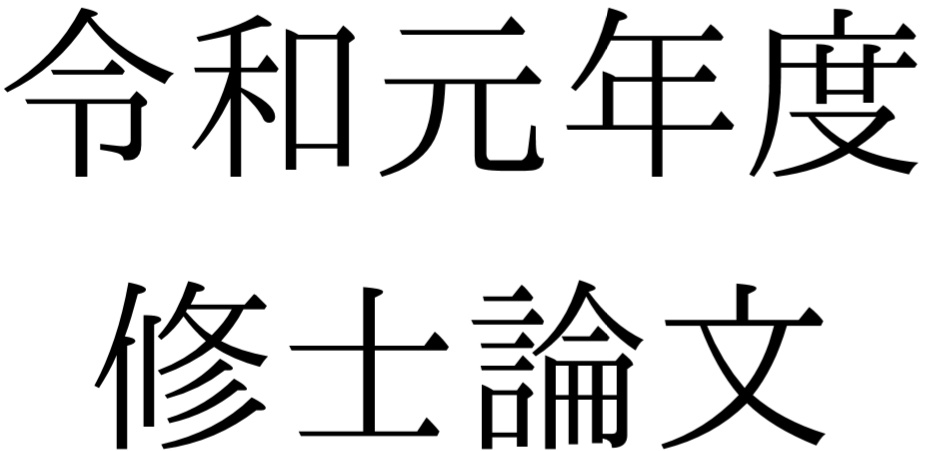
\includegraphics[width=4.0cm]{title.eps}
        \end{center}
    \end{figure}
    \vspace{2mm}
    {\LARGE\bf 題目 \par} 
    {\LARGE \textup Text Detection for Natural Scene based on \\MobileNet V2 and U-Net\par}
    \vspace{10mm}
    {\Large 報告者 \par}
    {\LARGE \quad 付\ 康为 \par}
    \vspace{10mm}
    {\Large 徳島大学大学院\ 先端技術科学教育部 \par}
    {\Large システム創生工学専攻\ 知能情報システム工学コース \par}
    \vspace{15mm}
    %------------------------------------------------------------------
    % 显示表格
    \begin{figure}[H]
        \begin{center}
            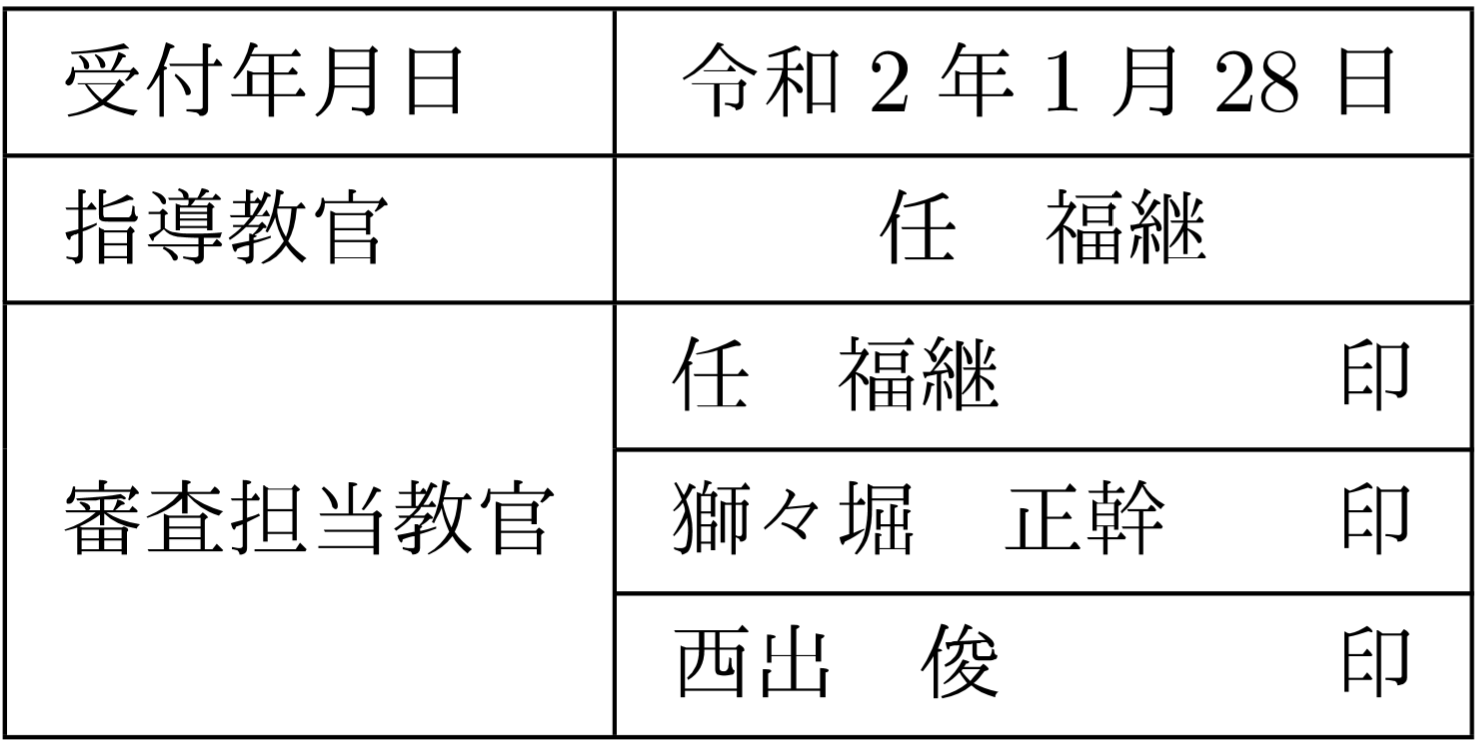
\includegraphics[width=8.0cm]{table.eps}
        \end{center}
    \end{figure}
\end{center}

\makeatother

\newpage % 分割页
\pagenumbering{roman}
\rhead{\thepage}
\cfoot{}
\tableofcontents % 目录
\newpage
\listoftables % 表格列表
\newpage
\listoffigures % 图片列表
\clearpage
\pagenumbering{arabic}

\begin{enabstract} % 摘要的内容
\addcontentsline{toc}{section}{Abstract} % 将摘要增加到目录中
\large % 设置
\lhead{Abstract} % 显示摘要的名称,即“Abstract”

% “\setlength\parindent{2em}”用于缩进
\setlength\parindent{2em} Detecting text areas in natural scenes can help us obtain significant text information from these complex and various natural scenes, which would provide great convenience for our daily life. For example, the computer vision systems on the vehicle are able to look for signposts on the highways, and detect the direction information on them instantly. It is beneficial to assisting vehicles in their autonomous driving operations. For computer vision systems, the image quality of natural scenes is easily affected by the lighting and the performance of image acquisition equipment. In addition, the background of natural scenes such as plenty of colors, scales, and text directions is extremely complex and has a large amount of image noise. Therefore, it is a great challenge for computer vision systems to detect text areas in natural scenes.

\setlength\parindent{2em} Recently, compared with traditional text detection methods, the accuracy of text detection based on deep learning has been improved greatly. However, with the purpose of improving the detect accuracy further, most of these text detectors which are based on deep learning applies large-scale neural network models, for example VGG or ResNet. Because these models own a huge number of parameters and their weight files are quite large (VGG model is over 500 MB, and ResNet model is about 100 MB), it is difficult to make them suitable for mobile devices that has limited computing ability, which limits the application of deep learning in our daily life.

\setlength\parindent{2em} The purpose of this article is to design a kind of text detector for natural scenes with low neural network complexity, which makes it feasible that the text detector could be used in all kinds of mobile platforms such as our smart phones. It would be very convenient for users to detect text areas in natural scenes using mobile phones. This text detector is on the basis of the small-scale neural network model called MobileNet V2, and U-Net that is commonly used in the research of image semantic segmentation. Firstly, this text detector extracts the text features from the natural scene image with the help of MobileNet V2. Second, U-Net is applied to classifying the pixels in this image, and the mask image of the text areas is generated. Then, some image processing algorithm on OpenCV, for example the enclosing rectangle and the minimum enclosing rectangle, can help us obtain the bounding boxes of mask areas and map these boxes onto the original image. Finally, the text areas in the natural scene have been detected.

\setlength\parindent{2em} The size of weight file of this neural network model designed by this paper is about 16 MB, and its number of parameters is quite small, which is suitable for running on mobile devices. In addition, this model has a great speed for text detection. This text detector solves the problems that general text detectors based on deep learning cannot be applied to mobile platforms with weak computer power. The experiment result based on the ICDAR 2013 dataset proves that this model has a good performance on the text detection for natural scenes. \\

% “\noindent”用于取消缩进,“\textbf”用于加粗字体
\noindent\textbf{Keywords:} Deep Learning, Natural scene, Text detection, MobileNet V2, U-Net

\end{enabstract}

\newpage

\lhead{\leftmark} % 取消“\lhead{Abstract}”的设置

\section{Introduction}

\large

\setlength\parindent{2em} The images of natural scene contain a wealth of information. With the continuous development of mobile device technology, more and more natural scenes are recorded and saved in the form of images. It has an important significance of research how to detect text areas in natural scenes based on computer vision systems, and how to obtain the most important text information from these images.

\subsection{Background and significance of research}

\subsubsection{Difficulties of text detection for natural scene}

\setlength\parindent{2em} More than 80\% of the information received by the human brain is through the human visual perception system, which is enough to prove the important role that images are playing in the process of human being's cognizance of the world [1]. Compared with some low-level information (such as position, outline, and color), the texts in complex natural scenes usually have specific semantic information, which attracts more people's attention [2].

\setlength\parindent{2em} Text detection for natural scenes has quite wide application foregrounds in many aspects:

\setlength\parindent{2em} (1) Assisted reading for the visually impaired: The visually impaired have many difficulties in reading and understanding the texts directly. The text detector is able to detect the texts from books or natural scenes in very short time. Then, the recognition operation is performed, and the text information is transmitted to the visually impaired in the form of speech.

\setlength\parindent{2em} (2) Autopilot technology: The text detection system can assist the vehicle to drive automatically on the highways [3]. Computer vision systems first gather natural scene information in the form of images on the car's driving direction, and then extracts some important text information from these images, such as the highway directions. This text information would be of great importance for helping the vehicle find the right highway direction.

\setlength\parindent{2em} However, detecting text areas from natural scenes has been a difficult problem in computer vision field all the time. The main reasons are given as follows:

\setlength\parindent{2em} (1) The text areas in natural scenes may have various sizes, colors or even types of characters. They may also have all kinds of patterns, for example the horizontal, vertical, or curved.

\setlength\parindent{2em} (2) Some text areas in natural scenes may appear to be incomplete or fuzzy. The more important thing is that, the image quality also has a great influence on the effectiveness of text detection.

\setlength\parindent{2em} (3) The natural scene image consists of text information and image background. The image background of natural scenes is very complex and even similar to the text areas, so it is quite difficult for computer vision systems to separate text areas from non-text areas, which makes segmentation and extraction of text areas from natural scenes a great challenge [4].

\setlength\parindent{2em} Fig 1.1 shows some text areas in the actual natural scenes, from which the difficulty of text detection for natural scenes could be really understood.

\begin{figure}[htbp] % 图片的显示
    \begin{center}
        % 设置图片的大小,与图片的路径
        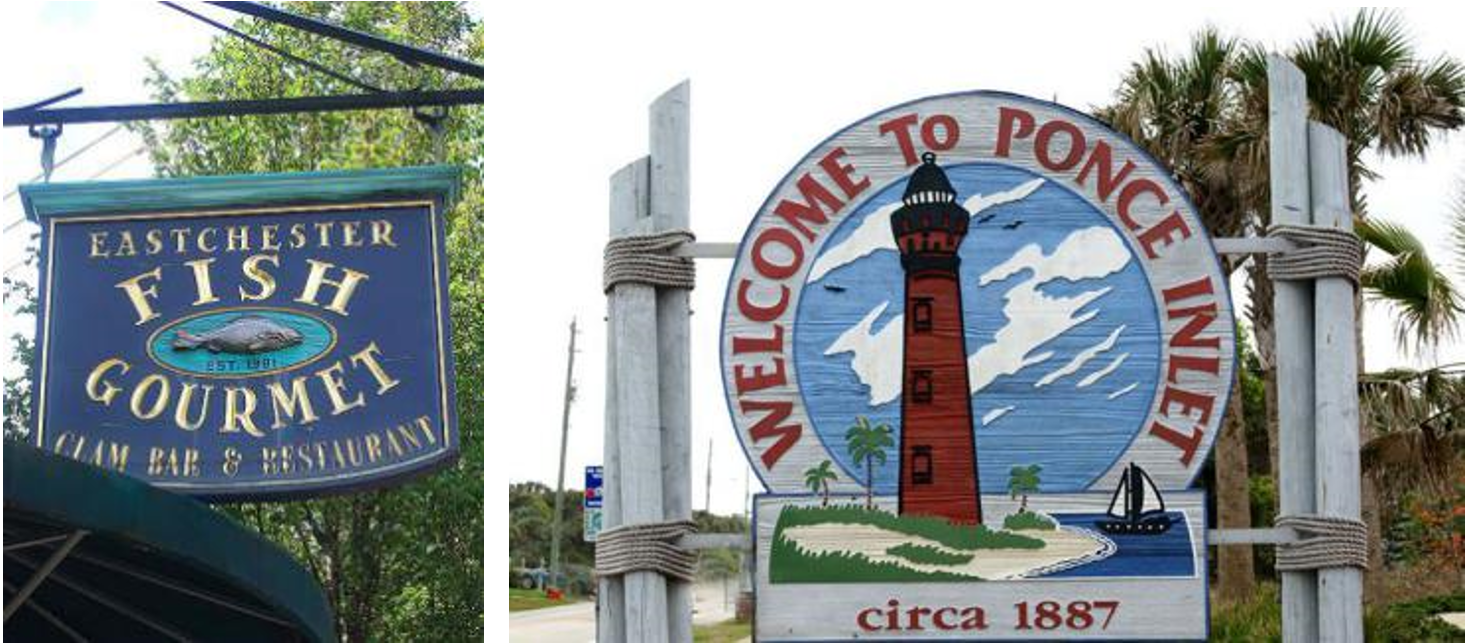
\includegraphics[width=12.5cm]{Paper_Images/1_1.eps}
    \end{center}
    \vspace{-3mm} % 减少图片与正文的间隔
    \caption{Text areas in actual natural scenes} % 图片的名称
    \vspace{-4mm} % 减少图片与正文的间隔
\end{figure}

\subsubsection{Necessity of lightweight text detector}

\setlength\parindent{2em} The emergence of deep learning provides a new method for the research of text detection for natural scenes. Large-scale neural networks have greatly improved the accuracy of text detection, far exceeding the traditional detection methods that are based on the text features [5]. For the aim of further improving the detection accuracy, researchers adopt deeper neural network models and more detection steps. It not only makes the task of text detection more complicated, but also requires more and more powerful computing hardware, which makes the efficiency of text detection lower [6]. As a matter of fact, these neural network models have consumed plenty of computing resources, and it is quite difficult to adopt them on the mobile platforms, which limits the application of deep learning in the daily life.

\setlength\parindent{2em} In order to reduce the neural network complexity of the text detector so that it could be applied to mobile devices with limited computing power, this paper designs a kind of lightweight text detector for natural scenes, which is on the basis of lightweight neural network called MobileNet V2 and semantic segmentation network named U-Net. It is able to detect text areas of different scales or colors, and it even has some effective result in the detection of curved text areas. This detection model does not only reduce the complexity of neural network, but also improve the speed of text detection greatly. This model could provide an example of the text detection for natural scene by the mobile devices.

\subsection{Related Work}

\subsubsection{Research status of text detection}

\setlength\parindent{2em} Text detection technology was applied to the optical character recognition (OCR) at first. OCR has the ability of scanning and analyzing the pages in the book, and obtaining text and layout information from them [7], as shown in Fig 1.2. This technology brought great convenience for the entry of text files, and it decreased the workload considerably for the typists. 

\begin{figure}[htbp]
    \begin{center}
        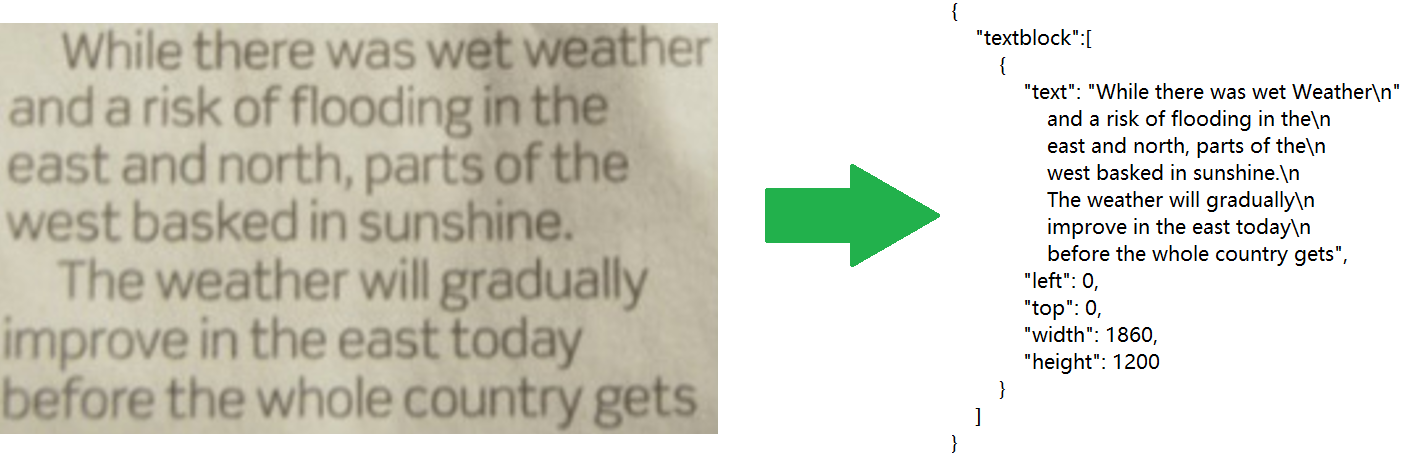
\includegraphics[width=15.0cm]{Paper_Images/1_2.eps}
    \end{center}
    \vspace{-3mm} % 减少图片与正文的间隔
    \caption{Optical Character Recognition}
    \vspace{-4mm} % 减少图片与正文的间隔
\end{figure}

\setlength\parindent{2em} Later, the computer vision researchers extended the field of text detection to natural scenes, hoping for extracting important text information from these complex natural scenes, so that computer vision systems could understand the semantic of natural scenes better. In the past, researchers used all sorts of traditional algorithms like SIFT, to extract texture features of text areas in natural scene images manually, such as the shape of text areas. A typical method is the MSER algorithm that is used by traditional text detectors [8]. The MSER algorithm has a great effect on the text detection when there is less noise in the natural scene image, as shown in Fig 1.3. However, in that case where the natural scene image has the complicated background, the MSER algorithm would make a lot of mistakes for the text detection.

\begin{figure}[htbp]
    \begin{center}
        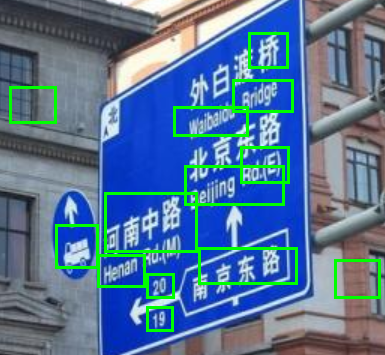
\includegraphics[width=8.5cm]{Paper_Images/1_3.eps}
    \end{center}
    \vspace{-3mm} % 减少图片与正文的间隔
    \caption{Example of text detection by MSER algorithm}
    \vspace{-4mm} % 减少图片与正文的间隔
\end{figure}

\setlength\parindent{2em} In recent years, the general object detection based on the deep learning has been achieving the remarkable results. Many efficient and effective object detectors have been invented with the assistance of deep learning technology, such as SSD, YOLO and Faster RCNN [9]. The researchers tried to introduce the deep learning into the task of text detection, and they regarded the text lines in the natural scene images as the common objects. Firstly, the text object is detected by the neural network model, and then with the help of sliding window method and NMS (Non-Maximum Suppression) algorithm that are commonly used in the general object detection, the text areas are located by those rectangle boxes of various sizes in natural scenes [10]. Compared with the MSER algorithm, its detection accuracy has been greatly improved. The well-known text detectors based on deep learning are CTPN and Fused Text Segmentation Networks.

\setlength\parindent{2em} CTPN is a text detection method based on Faster-RCNN. It applies VGG16 to extracting the text features from images, then detects multiple fixed-width text segments by the BLSTM model. CTPN connects these segments with each other for the purpose of forming the complete text lines, and then the text areas in the natural scenes are obtained [11]. The principle of CTPN is shown in Fig 1.4. CTPN is proved to have a great effect on text detection in the horizontal direction.

\begin{figure}[htbp]
    \begin{center}
        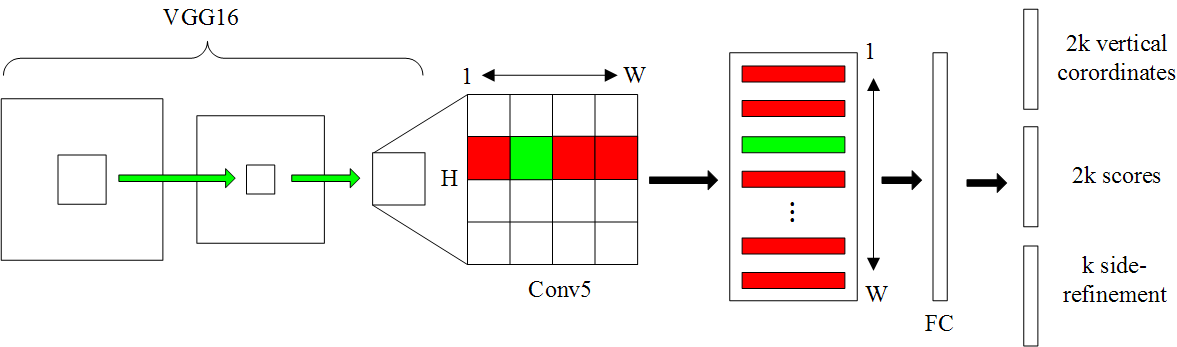
\includegraphics[width=15.0cm]{Paper_Images/1_4.eps}
    \end{center}
    \vspace{-3mm} % 减少图片与正文的间隔
    \caption{Principle of CTPN}
    \vspace{-4mm} % 减少图片与正文的间隔
\end{figure}

\setlength\parindent{2em} Fused Text Segmentation Networks model supplies a great idea for the detection of multi-directional text areas [12], and its principle is shown in Fig 1.5. Firstly, different with CTPN, Fused Text Segmentation Network uses ResNet to extract the text features. Second, the operation of semantic segmentation are performed and each pixel in this image is classfied. Then, this method performed the regression prediction for these text areas, and the position information of the text areas is obtained in the end.

\begin{figure}[htbp]
    \begin{center}
        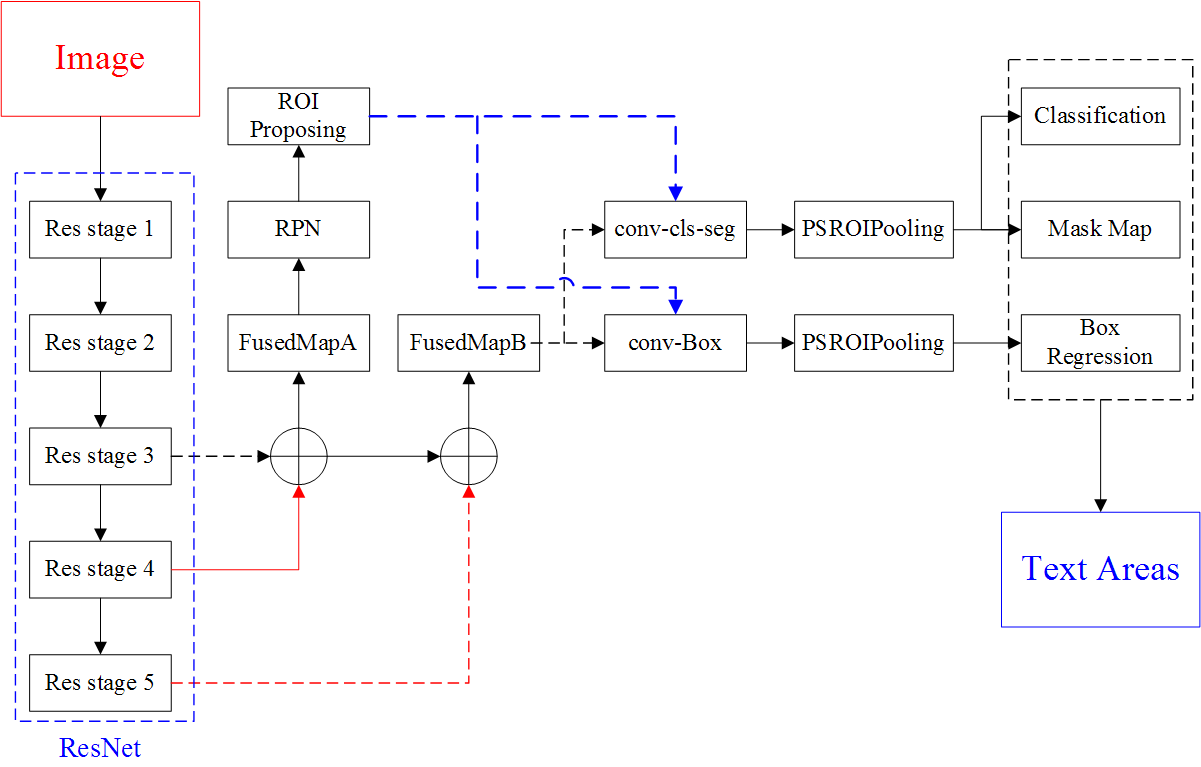
\includegraphics[width=14.5cm]{Paper_Images/1_5.eps}
    \end{center}
    \vspace{-3mm} % 减少图片与正文的间隔
    \caption{Principle of Fused Text Segmentation Network}
    \vspace{-4mm} % 减少图片与正文的间隔
\end{figure}

\subsubsection{Lightweight neural network}

\setlength\parindent{2em} Deep convolutional neural networks have raised the performance of computer vision systems to a new level. At the moment, most of researches about the neural network is toward building deeper and deeper networks, whose purpose is to improve the performance of neural networks further, such as the accuracy and recall [13]. It makes the neural networks own more and more convolutional layers or pooling layers, and the neural network model is more complicated than ever before [14]. Huge neural network model forces researchers to adopt more powerful computing resources. The computing power of common PC does no longer meet the requirement of large-scale deep learning, let alone mobile devices with extremely limited computing capabilities.

\setlength\parindent{2em} The first lightweight neural network model that achieves widespread application in mobile devices was MobileNet V1, which was developed by Google Corporation. This model uses depthwise separable convolutions that greatly reduces the number of parameters in deep neural networks with little loss on the performance [15]. The structure comparison between the depthwise separable convolution and the traditional convolution is shown in Fig 1.6. Suppose that the size of input feature map is $D_{F} * D_{F} * M$, and the size of output feature map is $D_{F} * D_{F} * N$, where $D_{F}$ represents the width and height of input feature map, the output feature map is the same as the input feature map, $M$ represents the channel number of input feature map, and $N$ is the channel number of output feature map; the size of convolution kernel is $D_{K} * D_{K}$. So the ratio of parameter number in the depthwise separable convolution to the one in the traditional convolution is:

\vspace{-2mm} % 减少公式与正文的间隔
\begin{equation} % 公式
\frac{D_K * D_K * M * D_F * D_F + M * N * D_F * D_F}{D_K * D_K * M * N * D_F * D_F} = \frac{1}{N} + \frac{1}{D_{k}^{2}}
\end{equation}

\vspace{2mm} % 减少公式与正文的间隔

\setlength\parindent{2em} It is obvious that the depthwise separable convolution reduces the parameter number of neural networks effectively. The MobileNet V1 model achieved the 70.6\% accuracy on ImageNet's Top-K classification competition, which is a great result.

\begin{figure}[htbp]
    \begin{center}
        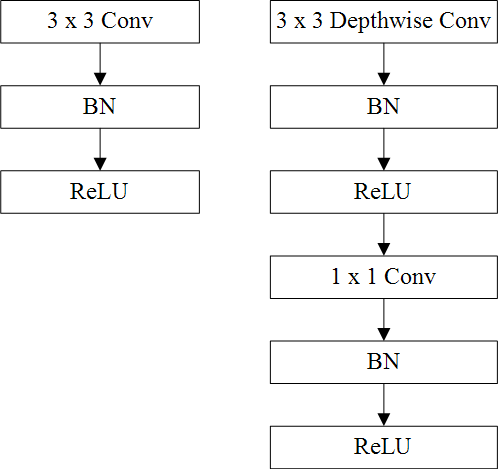
\includegraphics[width=7.5cm]{Paper_Images/1_6.eps}
    \end{center}
    \vspace{-3mm} % 减少图片与正文的间隔
    \caption{Traditional convolution (Left) and Depthwise separable convolution (Right)}
    \vspace{-2mm} % 减少图片与正文的间隔
\end{figure}

\setlength\parindent{2em} On the basis of MobileNet V1, Google developed a more efficient neural network model called MobileNet V2 afterwards [16]. This model introduces two kinds of new structures that are Inverted Residual and Linear Bottleneck. While reducing the neural network complexity, these structures also improve the processing speed of the neural network further at the same time. The structure of Inverted Residual and Linear Bottleneck are shown in Fig 1.7. The MobileNet V2 model achieved the 74.7\% accuracy on ImageNet's Top-K classification competition, which is better than the MobileNet V1 model. Currently, many mobile phone applications with object detection capabilities adopt the MobileNet V2 model. The feature extraction part of the neural network designed in this paper is based on the MobileNet V2 model as well.

\begin{figure}[htbp]
    \begin{center}
        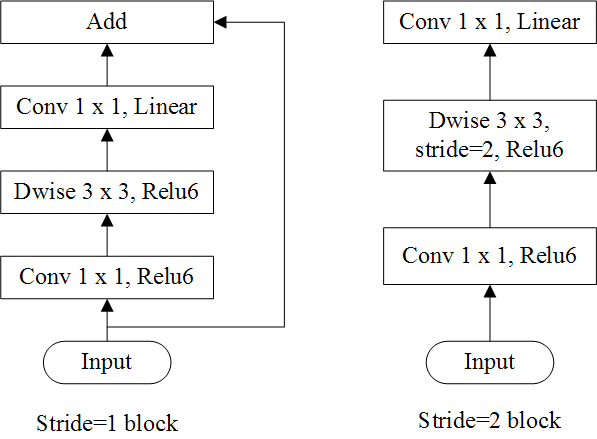
\includegraphics[width=8.5cm]{Paper_Images/1_7.eps}
    \end{center}
    \vspace{-3mm} % 减少图片与正文的间隔
    \caption{The structure of inverted residuals and linear bottleneck}
    \vspace{-4mm} % 减少图片与正文的间隔
\end{figure}

\subsubsection{Research status of semantic segmentation}

\setlength\parindent{2em} Image semantic segmentation is an important aspect of image understanding in the image processing and computer vision technology, and it is an important branch in the field of AI (Artificial Intelligence) as well [17]. The aim of image semantic segmentation is to classify each pixel in the image, then determine the category of each pixel, such as the background, person, or car, etc., which is shown in Fig 1.8. At present, the technology of image semantic segmentation is widely used in the research of autonomous driving and medical image analysis [18].

\begin{figure}[htbp]
    \begin{center}
        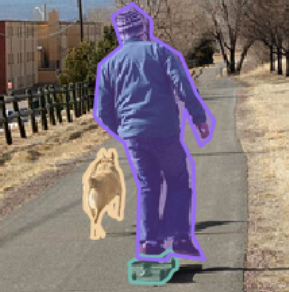
\includegraphics[width=6.5cm]{Paper_Images/1_8.eps}
    \end{center}
    \vspace{-3mm} % 减少图片与正文的间隔
    \caption{Image Semantic Segmentation}
    \vspace{-4mm} % 减少图片与正文的间隔
\end{figure}

\setlength\parindent{2em} In the field of medical image segmentation, U-Net is a popular semantic segmentation model, which has a great effect on the image binary segmentation. This model is suitable for the small-scale training dataset (About 30 pictures), and makes the training process not prone to overfitting. The more important thing is that U-Net has a fast image processing speed [19]. The entire structure of U-Net network is shown in Fig 1.9, which is similar to the English letter $U$.

\begin{figure}[htbp]
    \begin{center}
        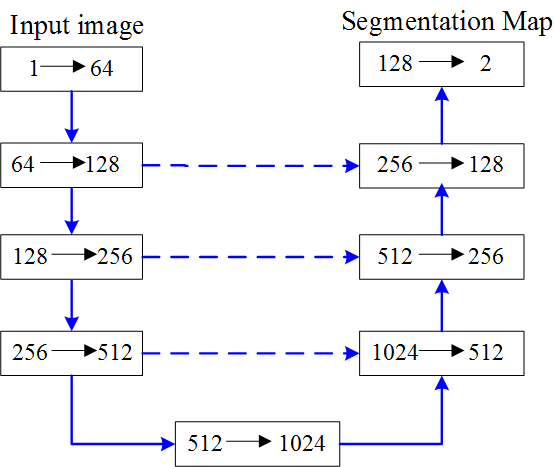
\includegraphics[width=11.5cm]{Paper_Images/1_9.eps}
    \end{center}
    \vspace{-3mm} % 减少图片与正文的间隔
    \caption{U-Net network structure}
    \vspace{-4mm} % 减少图片与正文的间隔
\end{figure}

\setlength\parindent{2em} U-Net first downsamples the input image multiple times by $Conv + Pooling$ operations, and then adopts $Deconv\ deconvolution$ to upsampling the feature map. At the same time, the feature map extracted from each layer is fused with the deconvolved ones. These operations are able to retain the detailed information in the original image effectively and prevent excessive loss of important semantic information [20]. The U-Net will output a feature map with the size of $388\ *\ 388\ *\ 2$, then we use the softmax function to process this feature map and achieve a semantically segmented image in the end. The softmax function is shown as follows:

\vspace{-2mm} % 减少公式与正文的间隔
\begin{equation} % 公式
y_{k} = \frac{exp(a_{k})}{\sum\limits_{i = 1}^{n}exp(a_{i})}
\end{equation}

\vspace{2mm} % 减少公式与正文的间隔

\noindent Where $exp$ represents the exponential function; $a_{k}$ is the k-th input signal for the output layer; $n$ represents the number of signals in the output layer; $y_{k}$ is the output of k-th neuron. The neural network model designed in this paper is also based on the U-Net neural network model.

\subsection{Thesis origination}

\setlength\parindent{2em} This paper is divided into 5 chapters, which is organized as follows.

\setlength\parindent{2em} Chapter 1: Introduction

\setlength\parindent{2em} In this chapter, we discuss the research background and significance of this paper. In addition, we conduct a detailed literature review of recent studies about text detection for natural scene, lightweight neural networks, and semantic segmentation. Also, the difficulties of text detection for natural scene are introduce briefly.

\setlength\parindent{2em} Chapter 2: Method of text detection for natural scene

\setlength\parindent{2em} In this chapter, we will show the general steps of text detection for natural scene, and briefly introduce a lightweight neural network model designed in this paper, which is based on MobileNet V2 and U-Net model. At the same time, a simple and fast method for locating text areas from the natural scene images is also introduced.

\setlength\parindent{2em} Chapter 3: Training process of the text detector

\setlength\parindent{2em} In this chapter, we first introduce the text detection dataset for natural scene used in the training process, and the method for data augmentation. Data augmentation is to solve the problem of overfitting during the training process. Then, the loss function that we adopt to training the neural network model is also showed.

\setlength\parindent{2em} Chapter 4: Experiments and analysis

\setlength\parindent{2em} In this chapter, we are going to perform experiments on the ICDAR 2013 natural scene text detection dataset, demonstrate the actual effect of text detection, and test the accuracy and speed of this text detector as well. The experimental results show that the model designed in this paper can achieve good results in text detection for natural scene with only little loss of accuracy. The model is able to detect horizontal and inclined text areas, even the curved text areas. In addition, the speed of text detection has been greatly improved.

\setlength\parindent{2em} Chapter 5: Conclusion and Future work

\setlength\parindent{2em} In this chapter, we are about to summarize the conclusions of this paper and discuss future work at the same time. Next, some improvements for this model are made to increase the speed and accuracy of text detection further.

\newpage

\section{Method of text detection for natural scene}

\subsection{Steps of text detection for natural scene}

\setlength\parindent{2em} The target of text detection for natural scene is to segment text areas from all kinds of natural scenes in order to obtain important text information. The pipeline of text detection proposed in this paper is shown in Fig 2.1, which is mainly made up of 4 parts:

\begin{figure}[htbp]
    \begin{center}
        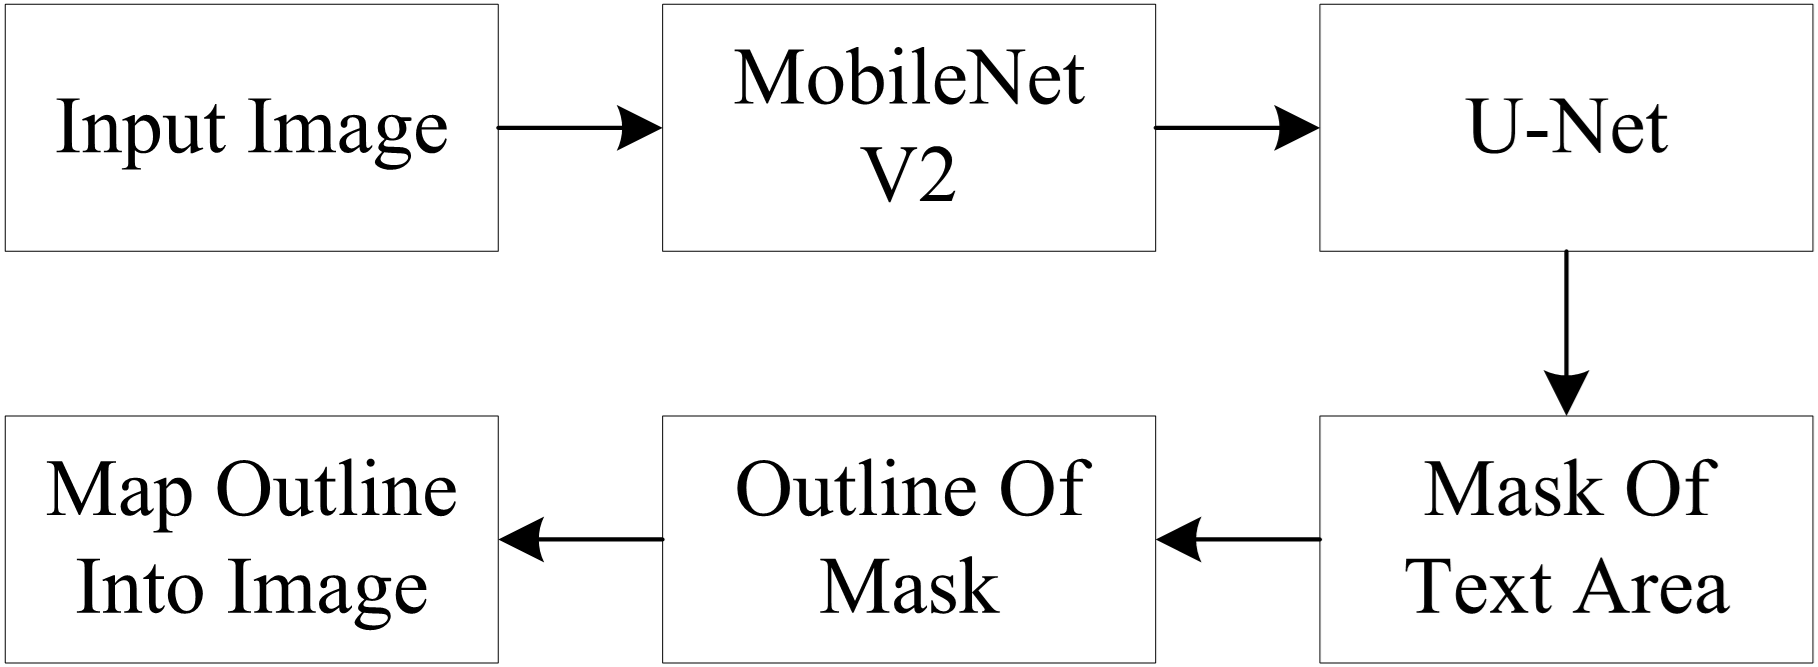
\includegraphics[width=11.5cm]{Paper_Images/2_1.eps}
    \end{center}
    \vspace{-3mm} % 减少图片与正文的间隔
    \caption{Pipeline of text detection proposed this paper}
    \vspace{-2mm} % 减少图片与正文的间隔
\end{figure}

\setlength\parindent{2em} (1) Feature extraction. First, the original image of natural scene is prepared, and then the MobileNet V2 neural network is used to extract the text features from this image automatically. Traditional text detectors such as the MSER and SWT extract the textural features with the help of LBP or SIFT algorithm [21]. The quality of such artificially extracted features is not high enough, and it is very easy for the text detector to mistake the text areas as the background of natural scene. The neural network owns the ability of extracting high-quality features from a large number of data automatically, improving the effectiveness of machine learning [22]. MobileNet V2 neural network model is able to extract high-quality texture features of text areas with few parameters, improving the effect of text detection for natural scene greatly.

\setlength\parindent{2em} (2) Semantic segmentation. The text features extracted by MobileNet V2 model is transferred to U-Net, and then the U-Net model will help us perform the semantic segmentation operation for the image, which is to determine whether each pixel belongs to the text area or not. The mask image of text areas will be generated by the neural network model designed in this paper eventually, which means cutting the text areas from the image of natural scene.

\setlength\parindent{2em} (3) Obtaining the outline of text areas from the mask image. The U-Net model generates the mask image of each character in the natural scene image. It is necessary to connect adjacent characters in order to form the complete text areas. Then, OpenCV applies to obtaining the minimum enclosing rectangles of each text area from the mask image, which is the outline of each text area.

\setlength\parindent{2em} (4) Mapping the outline of text areas onto the original image. The outline of text areas in the mask image is mapped onto the original image of natural scene, so the text areas in the original image are detected and obtained. The above steps implement the function of text detection for natural scene.

\subsection{Network architecture}

\setlength\parindent{2em} Inspired by the MobileNet V2 and U-Net, a lightweight text detector that is used for the natural scene is designed by this paper.

\setlength\parindent{2em}The MobileNet V2 neural network is transformed into the U-Net model, which is shown in Fig 2.2, just like the English letter $U$. And then we apply this model to classifying all pixels in the image of natural scene. The task of this neural network model is to detect the text areas, so all the pixels in this image are classified into two categories: pixels in the non-text areas or text areas. Finally, the neural network model will generate a mask image of the text areas.

\setlength\parindent{2em}The left half of the text detection model is based on the MobileNet V2 neural network, whose function is to extract the features of the text areas from the natural scene image automatically. At the same time, the MobileNet V2 is a lightweight feature extractor that is able to reduce the size of neural networks considerably. The feature maps extracted from each layer of the MobileNet V2 are fused with the right half part of this model, and then semantic segmentation operation is performed. At the end of this neural network model, the Tensor with shape $(224,\ 224,\ 16)$ is convolved, and a Tensor with shape $(224,\ 224,\ 2)$ is generated. In the end, an upsampling operation is performed to obtain the mask image of text areas.

\begin{figure}[htbp]
    \begin{center}
        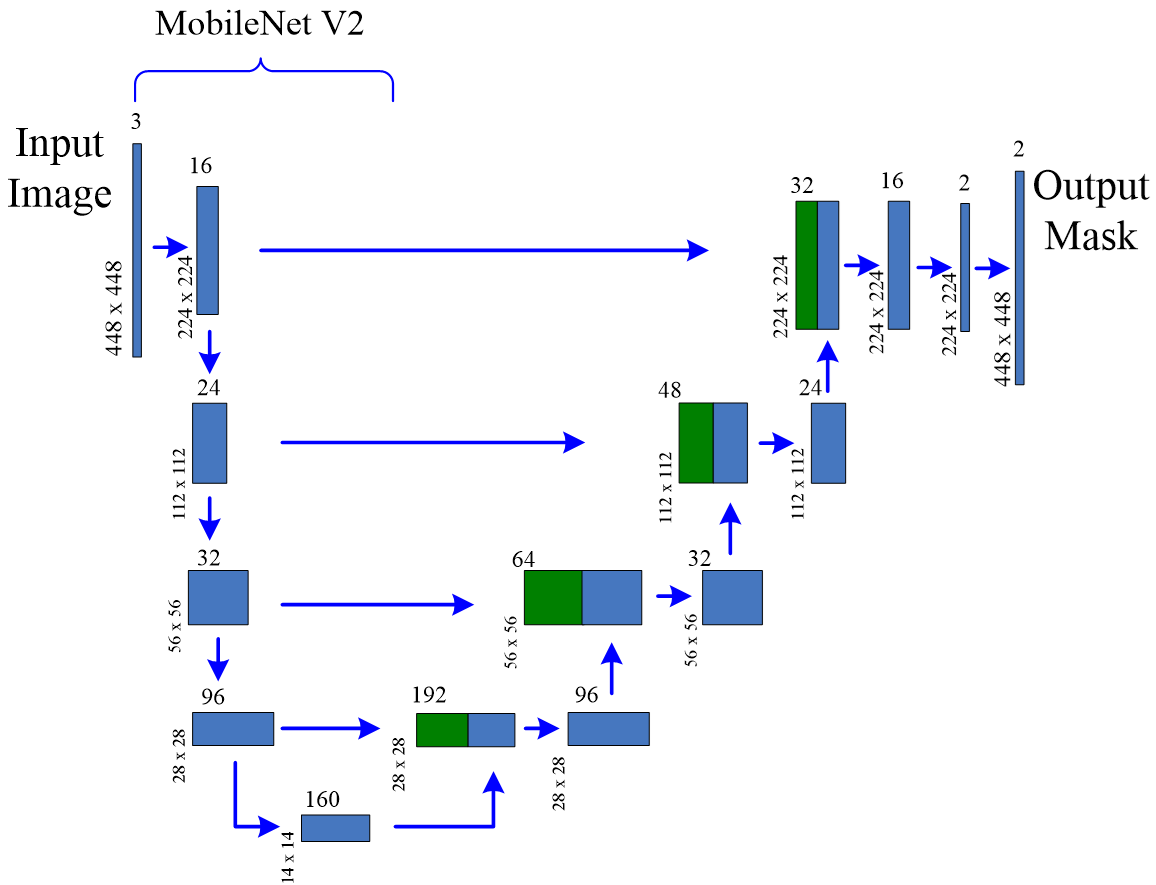
\includegraphics[width=13.5cm]{Paper_Images/2_2.eps}
    \end{center}
    \vspace{-3mm} % 减少图片与正文的间隔
    \caption{MobileNet V2 + U-Net neural network model}
    \vspace{-4mm} % 减少图片与正文的间隔
\end{figure}

\setlength\parindent{2em} FCN and U-Net are both neural network models used for the image semantic segmentation. However, FCN has the shortcoming of ignoring the features of small objects such as small texts, and the detection performance for small objects is not effective [23]. The above is the reason why FCN is not chosen as the feature extractor.

\setlength\parindent{2em} The neural network model designed in this paper makes the MobileNet V2 model send the features extracted from different bottleneck layers into the U-Net model, which makes sure that the features of text areas with different sizes can be extracted and the effect of text detection is improved greatly.

\subsection{OpenCV -- Tool of image processing}

\subsubsection{Introduction to OpenCV}

\setlength\parindent{2em} OpenCV is a cross-platform computer vision library that is developed by Intel Corporation [24]. It is suitable for many operation systems, for example Windows, Linux, and Mac OS. Even the embedded device platforms such as Android and IOS are able to use OpenCV to perform some image processing operations[25].

\setlength\parindent{2em} OpenCV supplies us with some useful function modules, which are shown as follows:

\begin{itemize}
\item Basic image processing: Image transformation such as deformation or perspective, linear or non-linear image filtering, color space conversion and background subtraction.

\item Basic object detection: Vehicle detection, face keypoint detection, and object tracking.

\item Graphic drawing: Draw some common graphics on the image, such as rectangles, circles, and texts [26].

\item Boundary detection: Detect the basic outline of objects, such as the enclosing rectangle, the minimum enclosing rectangle, and the minimum enclosing circle.

\item Machine learning: Provide some useful algorithms of machine learning, such as KNN algorithm, SVM algorithm.
\end{itemize}

\subsubsection{Enclosing rectangle}

\setlength\parindent{2em} In the actual image processing projects, there is often the demand to detect the outline of an object and the polygons on its periphery. Detecting these polygons will be of great value for us to analyze the images. The polygons used most commonly is the enclosing rectangle or minimum enclosing rectangle of an object. As shown in Figure 2.6, the green rectangular is the enclosing rectangle of the white area, while the blue rectangular is the minimum enclosing rectangle of the area.

\begin{figure}[H]
    \centering
    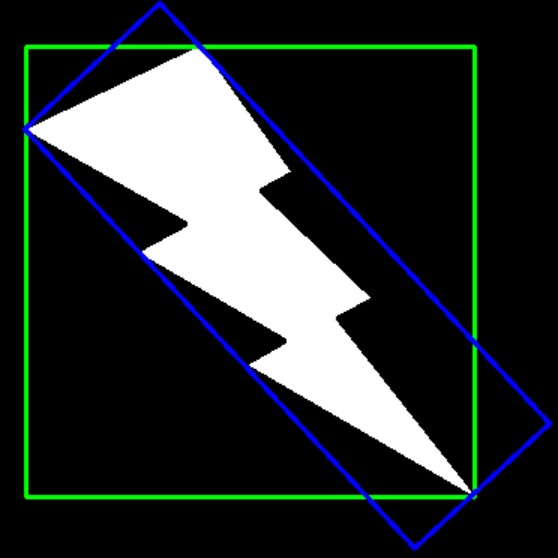
\includegraphics[width=8.0cm]{Paper_Images/2_6.eps}
    \vspace{-3mm} % 减少图片与正文的间隔
    \caption{The enclosing rectangle or minimum enclosing rectangle}
    \vspace{-4mm} % 减少图片与正文的间隔
\end{figure}

\setlength\parindent{2em} The algorithm for obtaining the enclosing rectangle of an object on the image is quite simple. The steps of this algorithm is shown as follows. Supposing that $PL$ is the point set of the object on this image, $PL_{i}$ is the element of $PL$.

\setlength\parindent{2em} The first step is to calculate the left top and the right bottom corners of this object through $PL$:

\vspace{-4mm} % 减少公式与正文的间隔
\begin{equation} % 公式
MinX = Min(PL_{i}.X)
\end{equation}

\vspace{-4mm} % 减少公式与正文的间隔
\begin{equation} % 公式
MinY = Min(PL_{i}.Y)
\end{equation}

\vspace{-4mm} % 减少公式与正文的间隔
\begin{equation} % 公式
MaxX = Max(PL_{i}.X)
\end{equation}

\vspace{-4mm} % 减少公式与正文的间隔
\begin{equation} % 公式
MaxY = Max(PL_{i}.Y)
\end{equation}

\vspace{-4mm} % 减少公式与正文的间隔
\begin{equation} % 公式
LeftTopPoint = (MinX,\ MinY)
\end{equation}

\vspace{-4mm} % 减少公式与正文的间隔
\begin{equation} % 公式
RightBottomPoint = (MaxX,\ MaxY)
\end{equation}

Therefore, the representation method of the enclosing rectangle $R$ is shown as follows:

\vspace{-4mm} % 减少公式与正文的间隔
\begin{equation} % 公式
R = (LeftTopPoint,\ RightBottomPoint)
\end{equation}

\setlength\parindent{2em} The minimum enclosing rectangle is the special enclosing rectangle with the smallest area for a set of points. The steps of this algorithm is shown as follows.

\setlength\parindent{2em} (1) Firstly, we need to calculate the enclosing rectangle of the object. The algorithm of enclosing rectangle has been introduced above.

\setlength\parindent{2em} (2) Second, the algorithm of making the area to be detected rotate a certain angle around a fixed point is necessary as well. Supposing that the point $(x_{1}, y_{1})$ is rotated around the other point $(x_{0}, y_{0})$ counterclockwise by the angle $A$, and the new point is $(x_{2}, y_{2})$:

\vspace{-4mm} % 减少公式与正文的间隔
\begin{equation}
x_{2} = (x_{1} - x_{0}) * cos(A) - (y_{1} - y_{0}) * sin(A) + x_{0}
\end{equation}

\vspace{-4mm} % 减少公式与正文的间隔
\begin{equation}
y_{2} = (x_{1} - x_{0}) * sin(A) + (y_{1} - y_{0}) * cos(A) + y_{0}
\end{equation}

\setlength\parindent{2em} (3) Third, it is necessary to rotate the area that is being detected with the interval of $1^{\circ}$ from $0^{\circ}$ to $90^{\circ}$. After every rotation of the area, we calculate the its corresponding enclosing rectangle, and record the area, vertex coordinates, and rotation degree of this rectangle.

\setlength\parindent{2em} (4) Then, we need to compare all enclosing rectangle obtained during the rotation process, and find a rectangle with the smallest area. In addition, the vertex coordinates and rotation angle of this rectangle are obtained as well.

(5) Finally, the enclosing rectangle need to be rotated. we rotate the enclosing rectangle with the smallest area obtained from the step 4 in the opposite direction (opposite to the direction in step 3) with the same angle. In the end, the minimum enclosing rectangle is obtained.

\subsubsection{Functions of OpenCV in this paper}

\setlength\parindent{2em} In this paper, OpenCV is adopted to achieving the following three functions for this text detector:

\setlength\parindent{2em} (1) Image pre-processing: OpenCV is used to augment the text detection dataset for the aim of solving the overfitting problem during the training process.

\setlength\parindent{2em} (2) Obtaining the outlines of text areas: OpenCV is going to help us frame the outlines of each character on the mask image, and the minimum enclosing rectangle of each text area as well.

\setlength\parindent{2em} (3) Mapping the outline of text areas onto the original image. The outline of text areas on the mask image is mapped onto the original image, which implements the positioning and detection of text areas in the natural scene.

\subsection{Location method of text areas}

\subsubsection{General object detection method based on deep learning}

\setlength\parindent{2em} The general object detection method based on deep learning uses rectangle boxes to locate the target objects commonly. The main process is shown in Fig 2.4:

\setlength\parindent{2em} (1) Firstly, we need to prepare an image to be detected, and send it to the pre-trained neural network model. The neural network model is able to generate a large number of candidate rectangular boxes which are used for selecting the possible locations of objects to be detected in the image [27].

\setlength\parindent{2em} (2) Second, these candidate rectangular boxes will be classified according to the types of objects to be detected. At the same time, the types of objects that each candidate rectangular boxes represents are marked as well [28].

\setlength\parindent{2em} (3) Then, these candidate rectangular boxes are filtered with the assistance of NMS (Non-Maximum Suppression) algorithm. For each item, only the candidate rectangular boxes with the highest probability of detection results are preserved [29].

\setlength\parindent{2em} (4) In the end, the preserved candidate rectangular boxes mark the locations of each object to be detected.

\setlength\parindent{2em} However, due to the multi-orientation and multi-scale of text areas on natural scenes, this method will produce plenty of candidate rectangular boxes with different sizes or angles by the neural network model. This generation of candidate rectangular boxes would consume a lot of computing resources, and also slow down the speed of text detection, which make it unsuitable for hardware platforms with limited computing power such as mobile devices.

\begin{figure}[H]
    \centering
        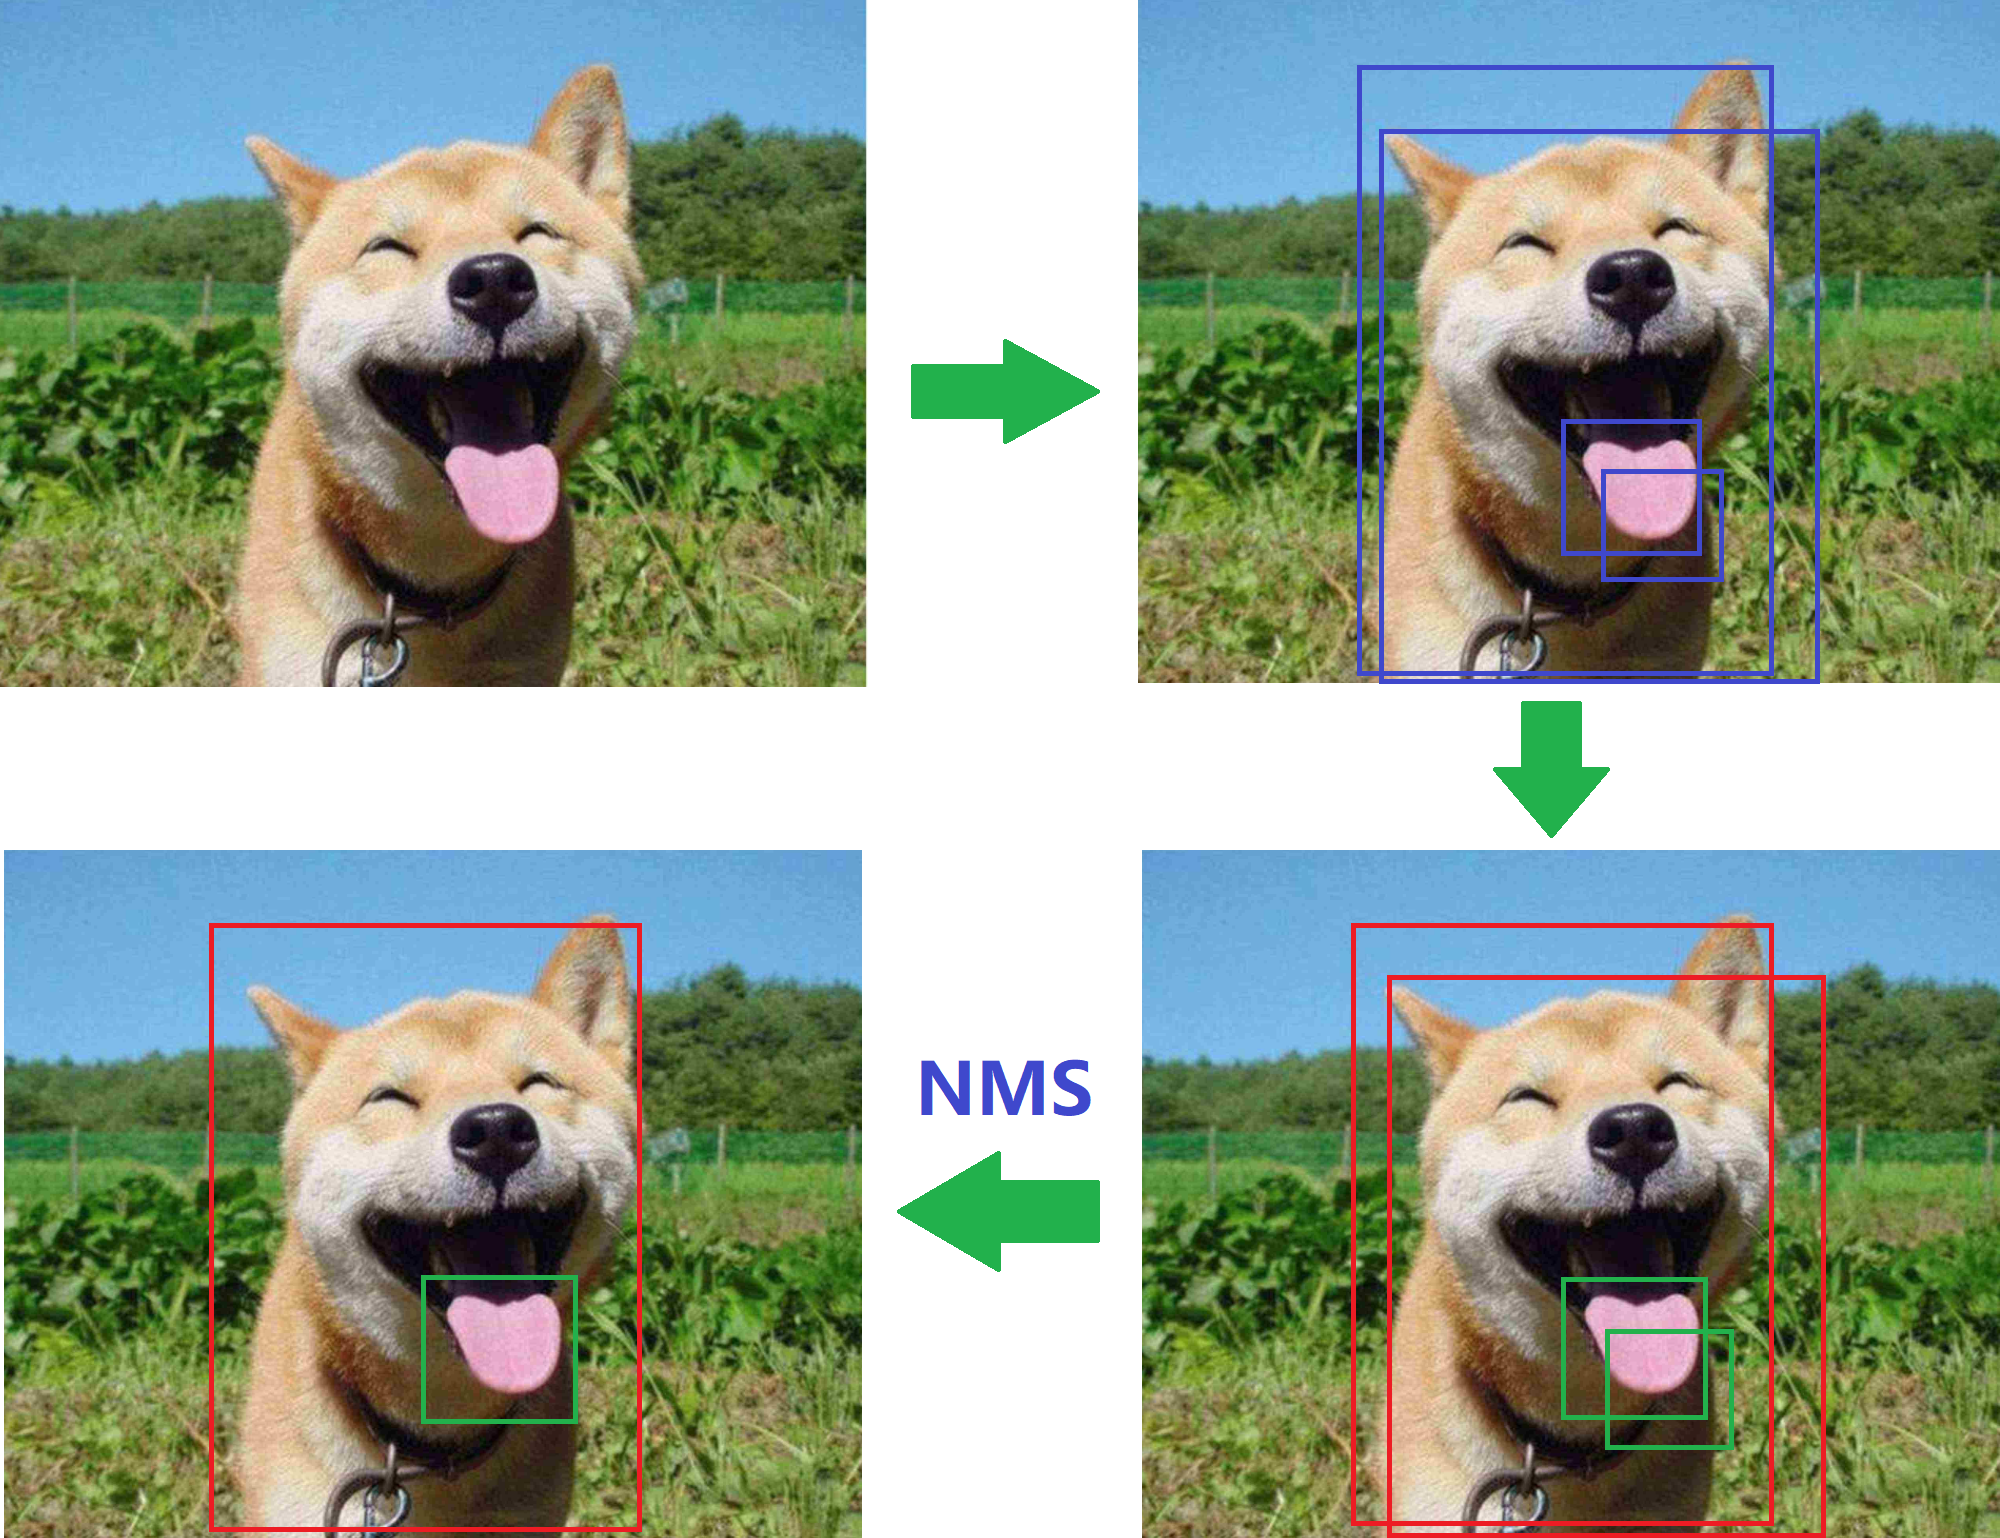
\includegraphics[width=11.0cm]{Paper_Images/2_4.eps}
    \vspace{-3mm} % 减少图片与正文的间隔
    \caption{Pipeline of the general object detection method}
    \vspace{-4mm} % 减少图片与正文的间隔
\end{figure}

\subsubsection{Our method for the location of text areas}

\setlength\parindent{2em} Instead of the general object detection method, a simple method for the text detection is designed by ourselves in this paper. The whole pipeline of this method is shown in Fig 2.5.

\setlength\parindent{2em} (1) Firstly, every character on the mask image is surrounded by the enclosing rectangles.

\setlength\parindent{2em} (2) Second, it is necessary to extend the boundary of these enclosing rectangles by 5 pixels, which makes adjacent enclosing rectangles contact with each other.

\setlength\parindent{2em} (3) Then, these rectangles are filled, and the algorithm of minimum enclosing rectangle is used to surround the filled areas.

\setlength\parindent{2em} (4) Finally, we map the outline of minimum enclosing rectangles onto the original image, so the text areas in the natural scene image are detected successfully.

\setlength\parindent{2em} This method above neither needs to generate a large number of candidate rectangular boxes, nor use the NMS algorithm to filter these candidate rectangular boxes. It is able to detect text areas quickly, and has a good detection effect on multi-orientation or multi-scale text areas.

\begin{figure}[H]
    \centering
    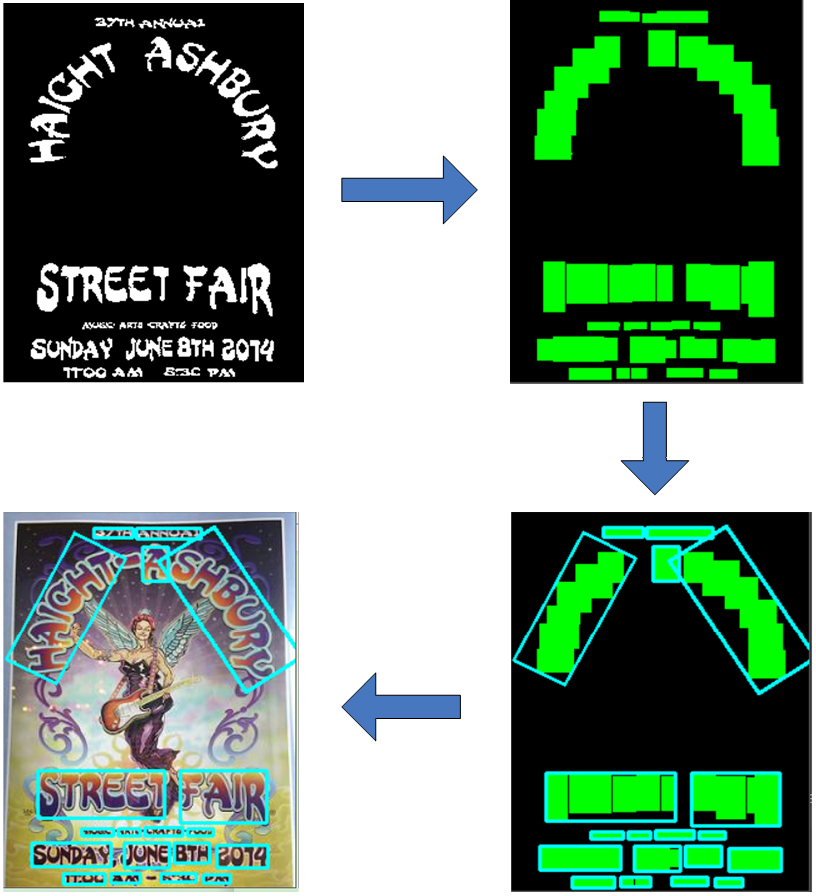
\includegraphics[width=9.5cm]{Paper_Images/2_5.eps}
    \vspace{-3mm} % 减少图片与正文的间隔
    \caption{Process of obtaining text areas}
    \vspace{-4mm} % 减少图片与正文的间隔
\end{figure}

\subsection{Chapter Summary}

\setlength\parindent{2em} In this chapter, the whole pipeline of text detection for natural scene are introduced in detail. 

\setlength\parindent{2em} A lightweight neural network model is introduced at first, whose function is to semantically segment images of natural scene. The structure of this model is on the basis of MobileNet V2 and U-Net.

\setlength\parindent{2em} Then, the powerful tool of image processing -- OpenCV is introduced briefly as well. This computer vision library will play an important role in the data augmentation and the location of text areas.

\setlength\parindent{2em} Finally, a simple and fast location method of text areas is designed by this paper. The method is able to locate text areas at the high speed, and detect multi-orientation or multi-scale text areas from natural scene image.

\newpage

\section{Training process of the text detector}

\subsection{Text detection dataset for natural scene}

\setlength\parindent{2em} At the moment, there are several public text detection datasets for natural scene, such as ICDAR 2013, ICDAR 2015, Total-Text and MSRA-TD500. The ways to label the location of text areas in these datasets are different: MSRA-TD500 supplies the inclination angle and the shape of text areas [30]; ICDAR 2015 supplies the coordinates of quadrilateral vertices of text areas [31]; Total-Text and ICDAR 2013 supplies the pixel-level mask image of text areas directly.

\setlength\parindent{2em} The experimental part of this paper needs the neural network model to classify all pixels on the natural scene image, and finally obtains the mask image of text areas, so the experiment is on the basis of Total-Text and ICDAR 2013 dataset.

\setlength\parindent{2em} Fig 3.1 shows the samples of ICDAR 2013 dataset. There are an original image and its corresponding mask image of the text areas for each sample in this dataset. According to the mask image, the colored pixels means the text areas and the white ares represent the background of natural scene [32]. The characters labeled are English or digits in ICDAR 2013 dataset, and most of them are horizontal.

\begin{figure}[H]
    \centering
    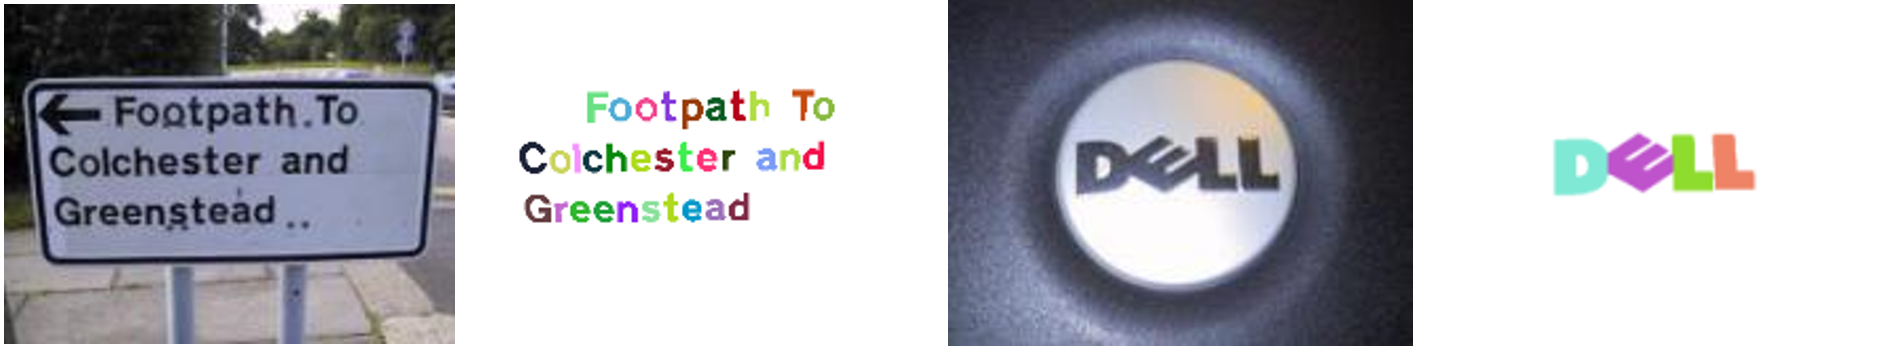
\includegraphics[width=14.5cm]{Paper_Images/3_5.eps}
    \vspace{-3mm} % 减少图片与正文的间隔
    \caption{ICDAR 2013 dataset samples}
    \vspace{-4mm} % 减少图片与正文的间隔
\end{figure}

\setlength\parindent{2em} Fig 3.2 shows the samples of Total-Text dataset. There are also an original image and its corresponding mask image of the text areas for each sample in Total-Text dataset. According to its mask image, the white pixels represent the text areas in the image, and the black areas represent the background of natural scene [33]. The text areas of this dataset are multi-directional, even some of them are curved. English or digits are labeled in this dataset.

\begin{figure}[H]
    \centering
    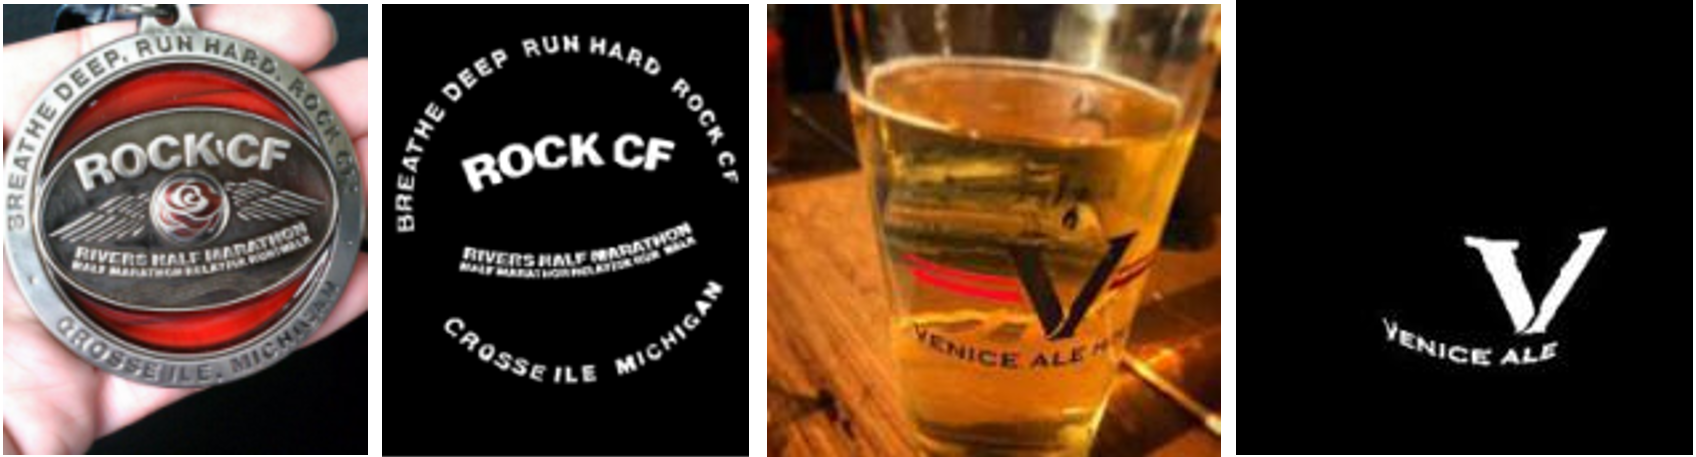
\includegraphics[width=14.5cm]{Paper_Images/3_6.eps}
    \vspace{-3mm} % 减少图片与正文的间隔
    \caption{Total-Text dataset samples}
    \vspace{-4mm} % 减少图片与正文的间隔
\end{figure}

\subsection{Data augmentation}

\subsubsection{Problem of the overfitting}

\setlength\parindent{2em} As a matter of fact, the quantity of samples in Total-Text dataset is quite small, as well as ICDAR 2013 dataset. For ICDAR 2013, this dataset contains 229 training images and 233 testing images; For Total-Text, there are only 1238 training images and 300 testing images in this dataset.

\setlength\parindent{2em} In case that there were few examples in the training dataset, the overfitting phenomenon will be easy to take place during the training process [34]. Overfitting is a difficult problem to solve for the deep learning. It means that the training effect of neural network model is quite excellent on the training dataset, while the effect on the testing dataset is not satisfactory. The specific phenomenon is that during the training process, the loss of neural network to the training dataset continues to decrease, while the loss to the testing dataset appears to increase suddenly during the process of decrease [35], which is shown in Fig 3.2.

\begin{figure}[htbp]
    \centering
    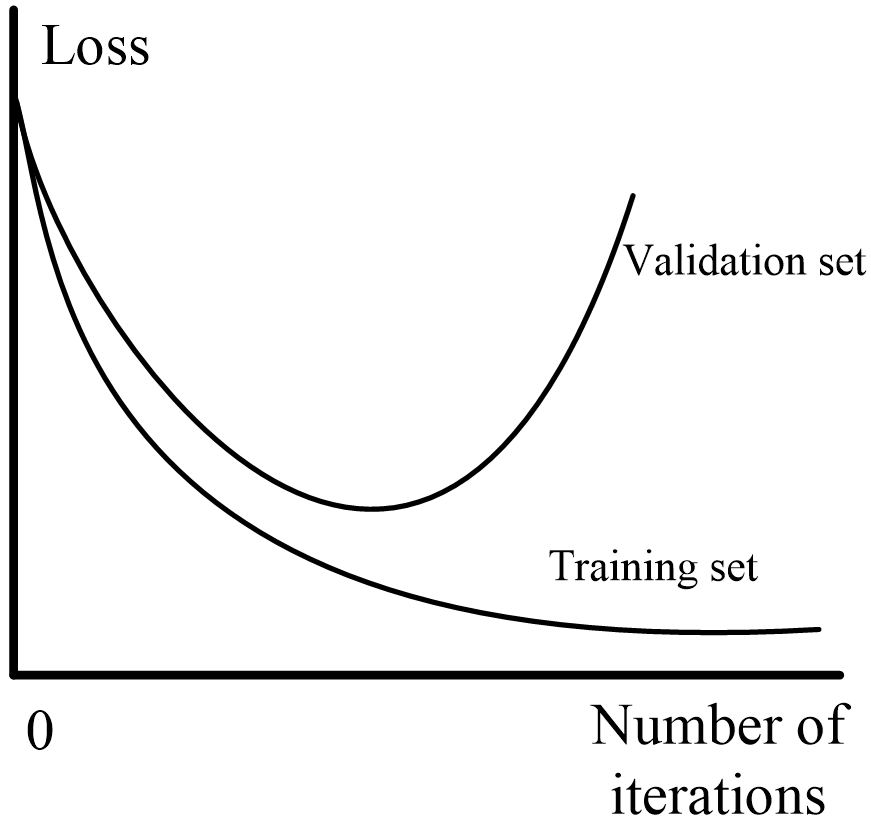
\includegraphics[width=6.5cm]{Paper_Images/3_2.eps}
    \vspace{-3mm} % 减少图片与正文的间隔
    \caption{Phenomenon of overfitting}
    \vspace{-4mm} % 减少图片与正文的间隔
\end{figure}

\subsubsection{Our method of data augmentation}

\setlength\parindent{2em} Augmenting the dataset is a common method for suppressing the overfitting problem [36]. In order to obtain as many training samples as possible, it is necessary to mix the Total-Text and ICDAR 2013 datasets: The training data is the whole Total-Text, and the training parts of ICDAR 2013 as well. There are 1767 samples in total, and we will perform the operation of data augmentation for these images afterwards. The testing data is the testing images of ICDAR 2013 dataset with a total of 233 samples.

\setlength\parindent{2em} However, only mixing the datasets with each other is not enough to solve the problem of overfitting considerably. So a new method of the data augmentation is come up with in this paper. The method of augmenting the dataset is to adopt a sliding window with size $(448,\ 448)$, which cuts the original image and the corresponding mask simultaneously, and then saves the part cut down from them as a new sample. We move the sliding window to the right, and cut the original image and the corresponding mask until the sliding window reaches the right edge of the image. Then, We move the sliding window down and repeat the above process. The whole process is shown in Fig 3.4.

\begin{figure}[H]
    \centering
    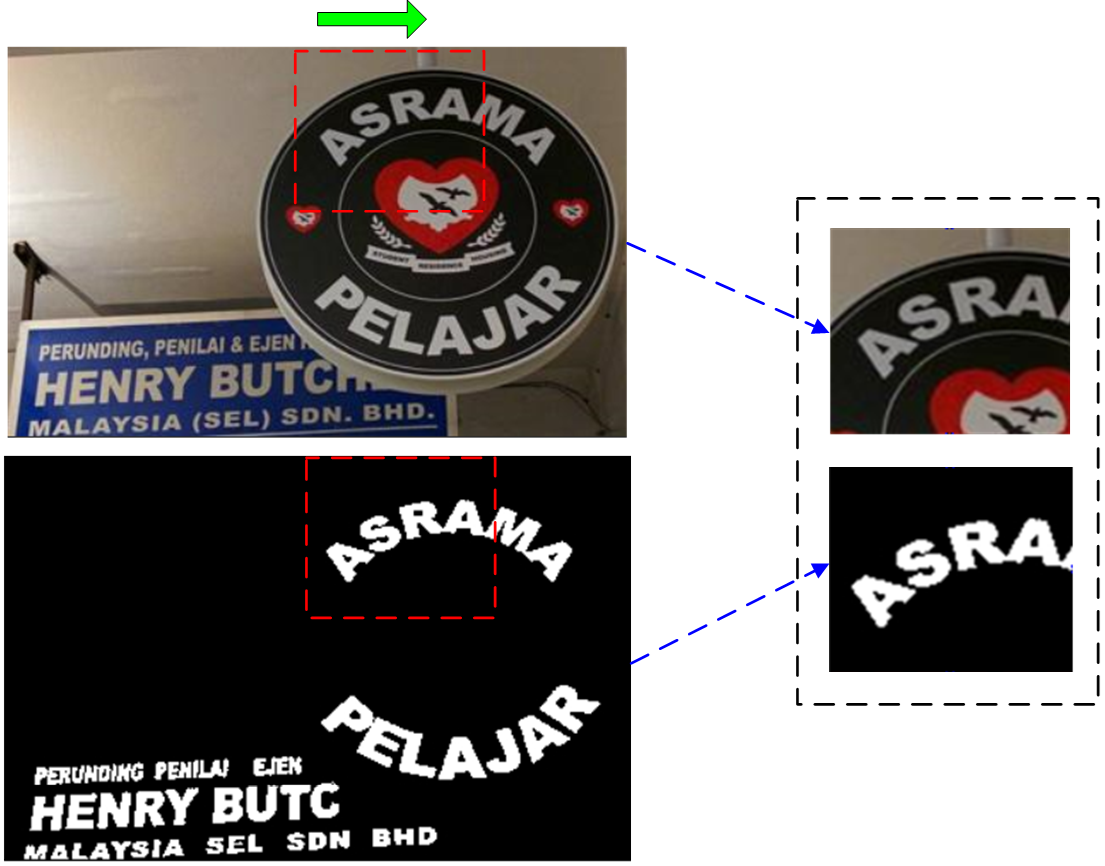
\includegraphics[width=8.5cm]{Paper_Images/3_3.eps}
    \vspace{-3mm} % 减少图片与正文的间隔
    \caption{Augmenting the dataset using a sliding window}
    \vspace{-4mm} % 减少图片与正文的间隔
\end{figure}

\setlength\parindent{2em} The effect of data augmentation for the datasets is shown in Fig 3.5. It is obvious that one training sample in the dataset could be used to generate multiple training samples by this method.

\begin{figure}[H]
    \centering
    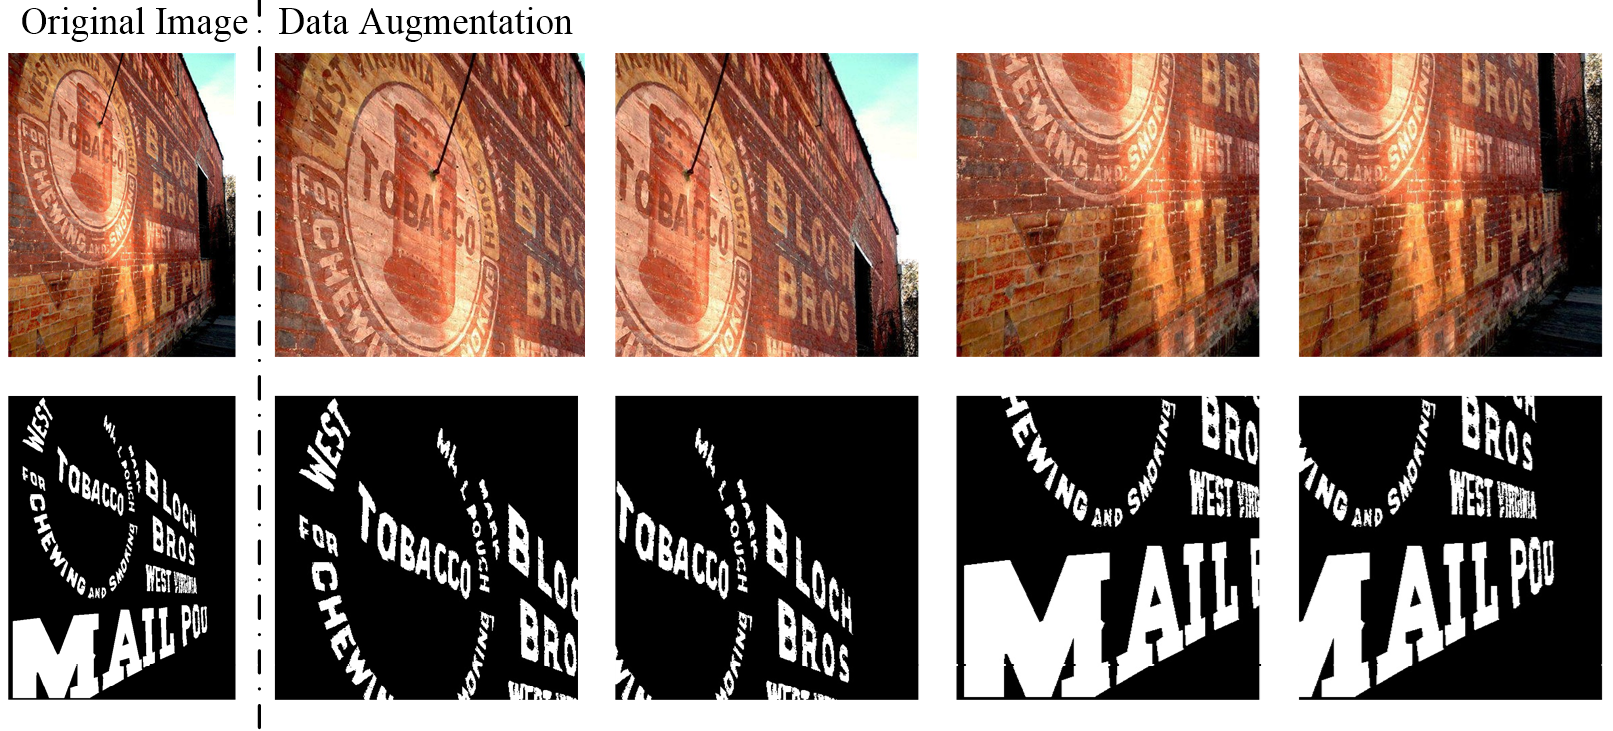
\includegraphics[width=14.5cm]{Paper_Images/3_4.eps}
    \vspace{-3mm} % 减少图片与正文的间隔
    \caption{Effect of data augmentation}
    \vspace{-4mm} % 减少图片与正文的间隔
\end{figure}

\subsection{Design of loss function}

\setlength\parindent{2em} In experiments, several loss functions were compared with each other, which are often used in the field of image semantic segmentation, such as Log loss, Dice Loss [37], BCE Loss, and their combinations [38]. In the end, it was found that when the loss function is a combination of BCE Loss and Dice Loss, the neural network model has the best training effect, and overfitting phenomenon is not easy to occur during the training process. The loss function is as follows:

\vspace{-2mm}

\begin{equation}
Loss(Y, \hat{Y}) = \frac{1}{N}\sum_{i = 1}^{N}(\frac{1}{2}Y_{i}log\hat{Y_{i}} + \frac{2Y_{i}\hat{Y_{i}}}{Y_{i} + \hat{Y_{i}}})
\end{equation}

\vspace{2mm}

\noindent where $N$ represents the number of training samples; $Y_{i}$ is the probability that the pixel is predicted to belong to text areas in the i-th sample; $\hat{Y_{i}}$ indicates the label of the i-th sample, that is, whether the pixel belongs to the text areas.

\subsection{Chapter Summary}

\setlength\parindent{2em} In this chapter, we first introduce the text detection datasets used for the experiment: Total-Text and ICDAR 2013.

\setlength\parindent{2em} Then, in order to solve the problem of overfitting that may take place during the training process, we propose a method of data augmentation to increase the number of samples in the text detection dataset.

\setlength\parindent{2em} In the end, a new loss function is designed, which is able to make the neural network fit better with the dataset.

\newpage

\section{Experiments and analysis}

\subsection{Experiment process}

\subsubsection{Experimental environment}

\setlength\parindent{2em} In terms of the experiment hardware, the CPU that is used has 6 cores, whose clock speed is 3.40 GHz; the size of RAM that the computer owns is 32 G, and the GPU being used is GeForce GTX TITAN X which has 12 G memory.

\setlength\parindent{2em} In terms of the experiment software, this experiment is performed on the CentOS operation system which is based on the Linux kernel. The programming language used in this experiment is Python. The construction of neural network model is on the basis of Pytorch that is a famous open source machine learning framework.

\subsubsection{Steps of this experiment}

\setlength\parindent{2em} The entire process of this experiment is shown in Fig 4.1:

\begin{figure}[htbp]
    \begin{center}
        \includegraphics[width=5.5cm]{Paper_Images/training.eps}
    \end{center}
    \vspace{-3mm} % 减少图片与正文的间隔
    \caption{Entire process of this experiment}
    \vspace{-4mm} % 减少图片与正文的间隔
\end{figure}

\setlength\parindent{2em} (1) First, the operation of data augmentation is performed for Total-Text and ICDAR 2013 datasets, which makes the sample size of training dataset expanded.

\setlength\parindent{2em} (2) Second, the neural network model and the loss function described above are constructed with the Pytorch framework.

\setlength\parindent{2em} (3) Then, the optimizer used for the training process is set to Adam.

\setlength\parindent{2em} (4) Finally, after setting the suitable batch size and epoch number, we start to train the neural network model using the GPU.

\setlength\parindent{2em} During the training process, TensorBoard is able to help us view the effects of neural network model training online, such as mask images generated by this model and the decrease process of loss value

\subsection{Image Semantic Segmentation}

\setlength\parindent{2em} The experiment results of image semantic segmentation are shown in Fig 4.2, where Fig 4.2(a) represents the original image of natural scene; Fig 4.2(b) is ground truth that is the manually labeled text areas in the dataset; Fig 4.2(c) is the text areas predicted by this neural network model. From these experiment results, it is obvious that the neural network model is able to generate the mask image of text areas based on the original image greatly.

\begin{figure}[htbp]
    \begin{center}
        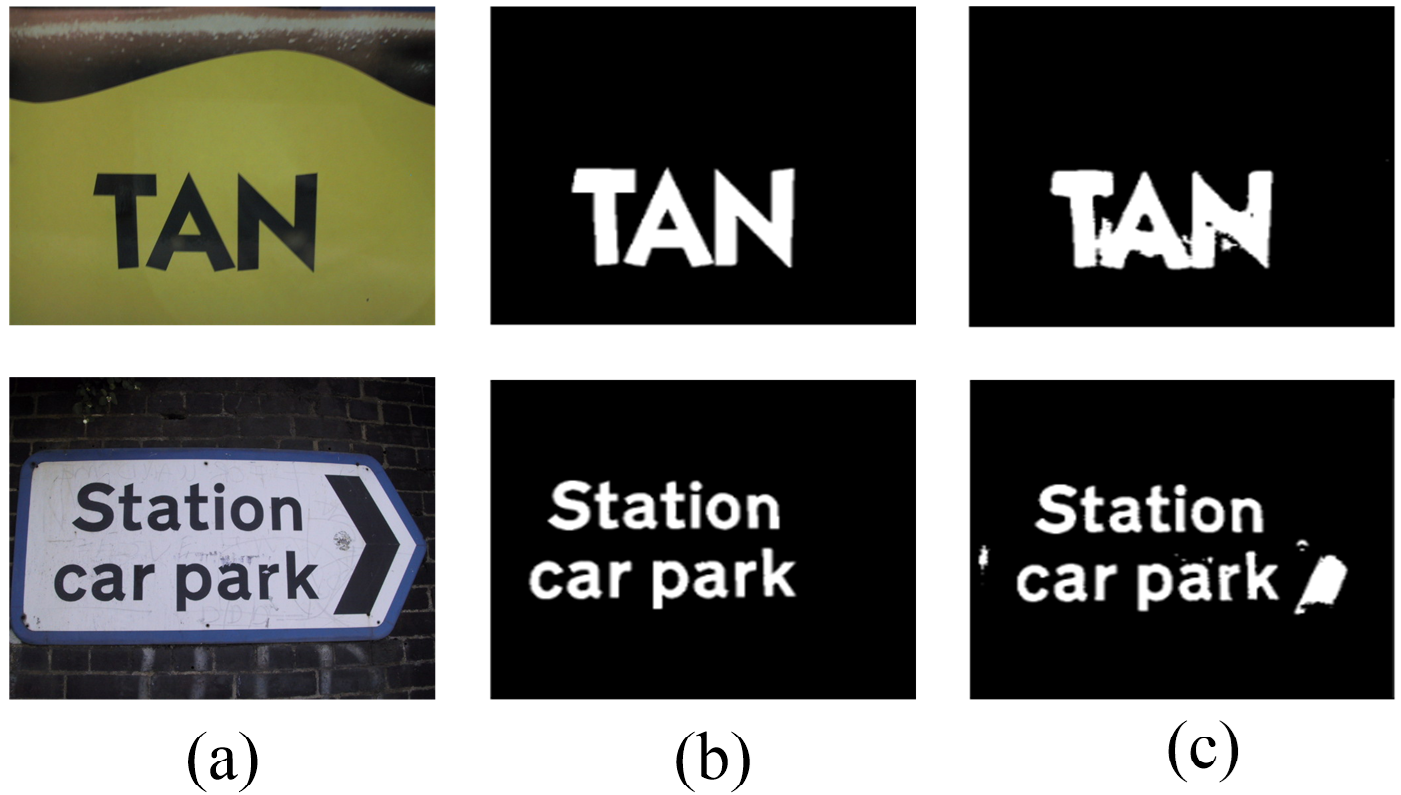
\includegraphics[width=12.0cm]{Paper_Images/4_1.eps}
    \end{center}
    \vspace{-3mm} % 减少图片与正文的间隔
    \caption{Neural network predicts the mask image of text areas}
    \vspace{-4mm} % 减少图片与正文的间隔
\end{figure}

\setlength\parindent{2em} However, the shortcomings of this neural network model can be also found from the experiment result: some pixels of the original image are classified incorrectly, for example some pixels of the background on the image are considered as pixels mistakenly in the text areas. The main reasons are that the scale of the neural network model is a little small relatively, the number of parameters in this neural network is quite few as well. This model is not as powerful as the large-scale neural networks such as VGG or Resnet, so the fitting effect on the training dataset is not very perfect. Moreover, even if the data augmentation operation is performed on the text detection dataset, the phenomenon of overfitting is only mitigated, and cannot be solved perfectly at present.

\subsection{Experiment of detecting text areas}

\setlength\parindent{2em} The example of text detection based on the method in this paper is shown in Fig 4.3.

\setlength\parindent{2em} It is obvious that this neural network model not only has a good effect on the text detection for the horizontal texts, but also is able to detect the text areas with multi-orientations. Even some curved text areas have been detected in these images successfully. The color of text areas has less influence on the effect of text detection. This method also has the ability of detecting the text areas with different sizes in natural scene images.

\begin{figure}[htbp]
    \begin{center}
        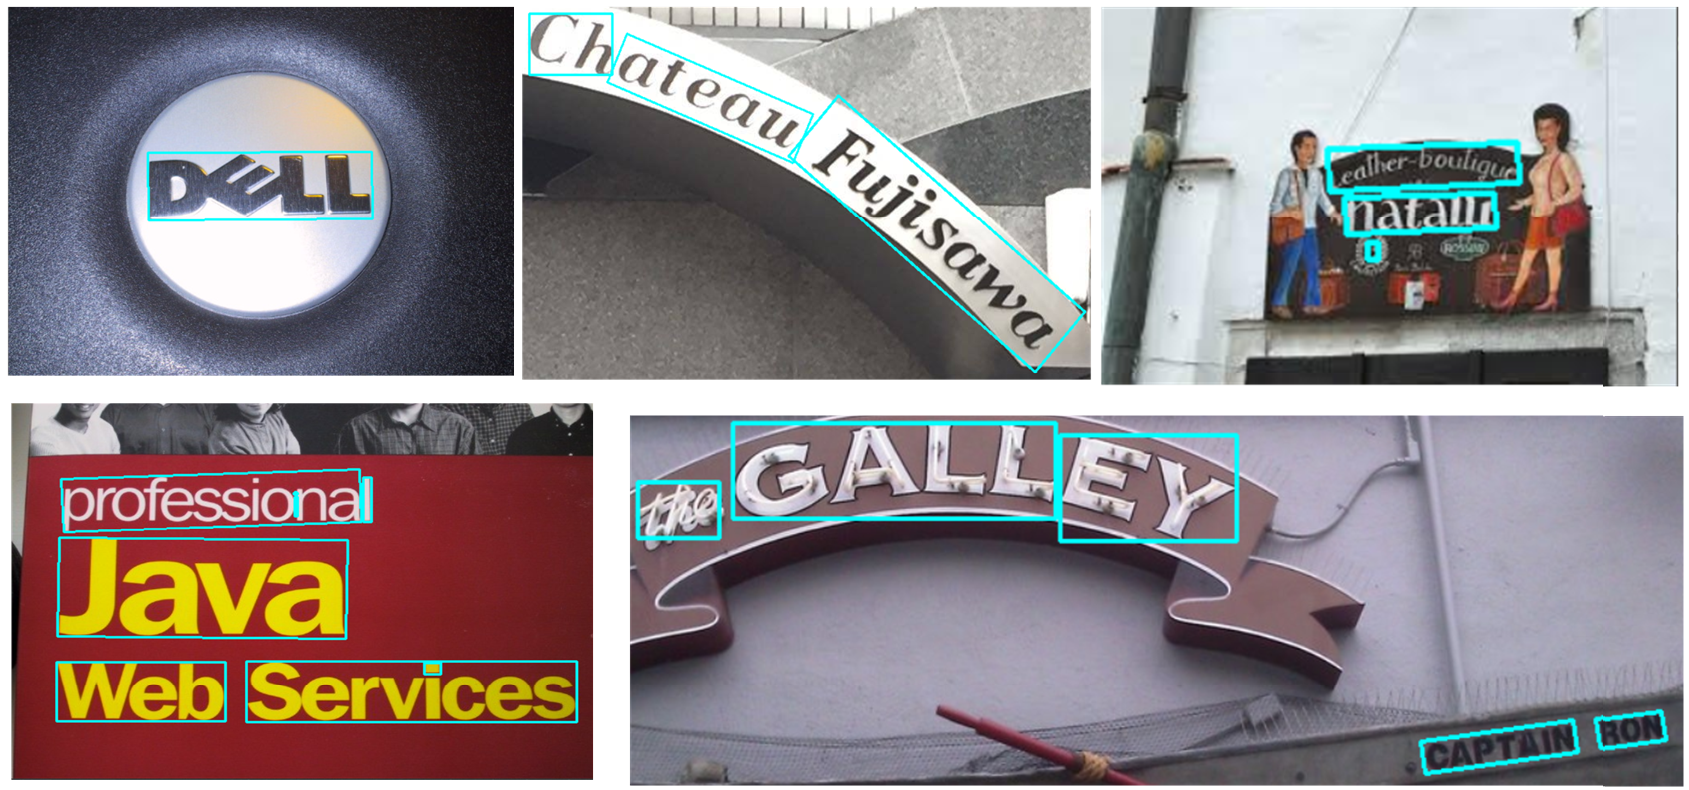
\includegraphics[width=13.5cm]{Paper_Images/4_2.eps}
    \end{center}
    \vspace{-3mm} % 减少图片与正文的间隔
    \caption{Example of text detection for natural scene}
    \vspace{-4mm} % 减少图片与正文的间隔
\end{figure}

\setlength\parindent{2em} As a matter of fact, this method is not perfect. Some drawbacks of this method are also obvious from Fig 4.3. For example, Some complete text areas are divided into multiple ones, such as $GALLEY$ which is divided into $GALL$ and $EY$ by this method. In fact, $GALLEY$ is the whole text area in the Total-Text dataset.

\setlength\parindent{2em} Moreover, the effect of text detection will be largely affected by the results of image semantic segmentation. If there is a remarkable difference between the text areas of the original image and the ones of mask image after the semantic segmentation, the final effect of text detection will be basically unsatisfactory.

\subsection{Comparison with other methods}

\setlength\parindent{2em} The innovation of this paper is to reduce the complexity of neural network, so it is necessary to compare with other text detection methods based on deep learning.

\setlength\parindent{2em}The comparison result is shown in Tab 4.1. In the task of object detection, Precision, F-score, and Recall, these three indicators are often used to evaluate the actual effect of the detection. An explanation of these indicators is shown in Figure 4.4.

\begin{figure}[htbp]
    \begin{center}
        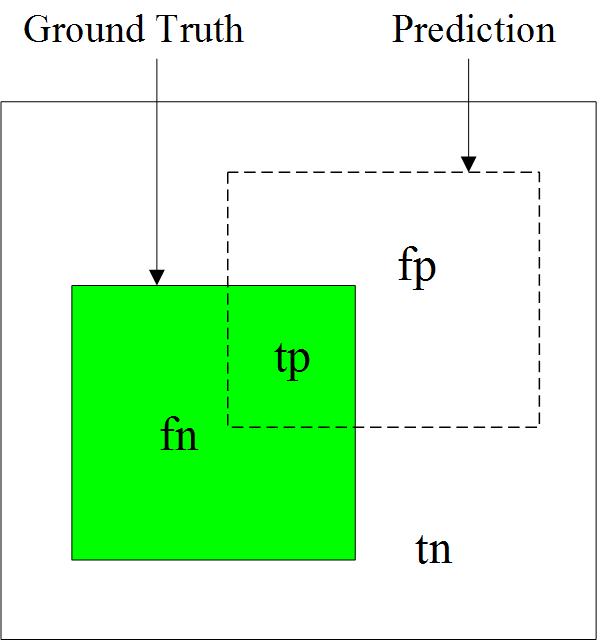
\includegraphics[width=8.0cm]{Paper_Images/standard.eps}
    \end{center}
    \vspace{-3mm} % 减少图片与正文的间隔
    \caption{Comparison standard}
    \vspace{-4mm} % 减少图片与正文的间隔
\end{figure}

\noindent Where $Ground\ Truth$ means manually labeled text areas, while $Prediction$ means text areas predicted by the text detector. The calculation methods for these three indicators are as follows:

\vspace{-2mm} % 减少公式与正文的间隔
\begin{equation} % 公式
Precision = \frac{tp}{tp + fp}
\end{equation}

\vspace{-2mm} % 减少公式与正文的间隔
\begin{equation} % 公式
Recall = \frac{tp}{tp + fn}
\end{equation}

\vspace{-2mm} % 减少公式与正文的间隔
\begin{equation} % 公式
F = \frac{2 * Recall * Precision}{Recall + Precision}
\end{equation}

\vspace{2mm} % 减少公式与正文的间隔

\setlength\parindent{2em} Compared with other text detection methods, the method that we propose in this paper has a slight loss in the accuracy, such as recall, precision, and F-score. However, it could generate the smaller weight file, and have the less complexity of neural network. At the same time, this method have the great speed of text detection. Therefore, this model can be applied to devices with limited computing capabilities such as smartphones. With respect to the data of weight size, we obtained them from the related repositories on github; For Liu [41] and Zhang [42], we inferred their weight size from the VGG model that they have used.

\begin{table}[!htbp]

\begin{center}
    \renewcommand\arraystretch{1.5}
    \begin{tabular}{|c|c|c|c|c|c|}
        \hline
        \multicolumn{6}{|c|}{ICDAR 2013 Dataset}                                                              \\ \hline
        & Recall        & Precision     & F-score       & Time (s)      & Weight Size (Mb) \\ \hline
        Proposed method    & 0.72          & 0.83          & 0.76          & \textbf{0.05} & \textbf{16}      \\ \hline
        TextBoxes {[}39{]} & 0.74          & 0.86          & 0.80          & 0.09          & 91               \\ \hline
        SSD {[}40{]}       & 0.60          & 0.80          & 0.68          & 0.10          & 90               \\ \hline
        CTPN {[}19{]}      & 0.73          & \textbf{0.93} & 0.82          & 0.14          & 78               \\ \hline
        Liu {[}41{]}       & \textbf{0.78} & 0.79          & 0.78          & 0.06          & $\approx$ 500    \\ \hline
        Zhang{[}42{]}      & \textbf{0.78} & 0.88          & \textbf{0.83} & 2.1           & $\approx$ 500    \\ \hline
    \end{tabular}
    \caption{Comparison of different text detection methods based on deep learning}
\end{center}
\end{table}

\subsection{Chapter Summary}

\setlength\parindent{2em} In this chapter, we conducted some experiments on the text detection method designed in this paper. The main experiment process is as follows.

\setlength\parindent{2em} First, the hardware and software used in this experiment were described in detail, such as the framework of machine learning called Pytorch and the GPU used for training the neural network model.

\setlength\parindent{2em} Next, we showed the semantic segmentation effect of this neural network model. It is obvious that the model could generate the mask image of text areas very well, and segment these text areas from the natural scene successfully.

\setlength\parindent{2em} Then, the examples of detecting text areas are shown as well. It is clear that this text detection method has a good detection effect on text areas with different sizes, colors, and multi-orientations.

\setlength\parindent{2em} In the end of this chapter, the comparison was made between this text detection method and other ones. The experiment proved that the the method we proposed was able to detect text areas from natural scenes quickly and accurately. The more important things were that it only took up very few hardware resources.

\newpage

\section{Conclusion and future work}

\subsection{Conclusion}

\setlength\parindent{2em} Images of natural scenes contain rich information, and texts in images have the rich semantic information. Texts are of great value to assist people in understanding the image and obtaining the key information. Therefore, the technology of text detection for natural scene has the important research value. In addition, the text detection technology also has a wide range of applications in the fields of information retrieval, assisting the visually impaired, industrial automation and intelligent transportation system.

\setlength\parindent{2em} This article first reviews the research significance of text detection for natural scene, and then introduces the research progress of text detection based on deep learning. The principles of these text detection methods are introduced briefly as well. We point out that these methods are too complicated and the neural network models they used is so large. In order to solve these shortcomings, this paper proposes a lightweight text detector for natural scene. The specific work is as follows.

\setlength\parindent{2em} (1) This model is on the basis of MobileNet V2 and U-Net neural network. Its function is to perform the operation of semantic segmentation on natural scene images and classify their pixels into two categories: text or non-text areas. This model not only reduces the complexity of neural network model greatly, but also accelerates the speed of text detection.

\setlength\parindent{2em} (2) The traditional method for object detection is that the neural network model first generates a large number of candidate rectangular boxes on the image, and then applies the NMS algorithm to filtering these boxes. This paper proposes a simple text area positioning method which just adopts the enclosing rectangle and the minimum enclosing rectangle used in the image processing field commonly. This method doesn't need to generate plenty of candidate rectangular boxes, thus further accelerates the speed of text detection and reduces the consumption of computing resources.

\setlength\parindent{2em} (3) Because the text detection datasets Total-Text and ICDAR 2013 used in this experiment are very small, and the number of samples in them is quite few, it is easy to cause the overfitting problem during the training process. So this paper designs a method for the data augmentation: we use a sliding window with the size $(448,\ 448)$ to cut the original image and its corresponding mask image in the dataset, which will generate a new sample for the dataset. This method is able to generate a large number of training samples from the small datasets, so as to alleviate the overfitting phenomenon during the training process.

\setlength\parindent{2em} (4) In order to make the neural network model fit better with the dataset, and improve the accuracy of semantic segmentation, a new loss function is designed in this paper. This loss function is a combination of BCE Loss and Dice Loss, which can make the neural network model own the great performance.

\subsection{Future work}

\setlength\parindent{2em} In this paper, we research the method of text detection for natural scene and make a lot of improvements. Although some achievements have been made, there are still some shortcomings. The new research would make further improvements from the following aspects:

\setlength\parindent{2em} (1) Improving the effect of semantic segmentation. In the whole process of text detection, the image semantic segmentation is a crucial step. However, it could be found from the actual effect that there are still pixels that have not been classified correctly. Therefore, some adjustments need to be made for the architecture of this neural network model.

\setlength\parindent{2em} (2) Detection for multiple types of text areas. At present, this method has the great limitations on different kinds of texts from natural scenes. Until now, only the datasets of text mask areas for English and digits have been found, which makes this method suitable for detecting English and digits in natural scenes merely. In the future, we would continue collecting the information of text detection datasets in order to find the useful ones for other kinds of texts. Even it is the nice idea to modify the model for making it applicable to the annotation methods of other text detection datasets.

\setlength\parindent{2em} (3) In fact, the method of using the minimum bounding rectangle to surround the text areas is not perfect. There are many curved text areas in natural scenes, and the minimum bounding rectangles that surround the text areas not only contain the text area information, but also the unnecessary background, which affects the accuracy of text detection enormously and has some influence on it. This method would be optimized for improving the detection of curved text areas.

\newpage

\section*{Acknowledgement} % 致谢
\addcontentsline{toc}{section}{Acknowledgement} % 将致谢添加到目录
\lhead{Acknowledgement} % 页眉的左边显示Acknowledgement

\setlength\parindent{2em} Time flies! The exchange life of one year at Tokushima University is quite short. During this short one-year period, I worked with other students of A1 group to study research problems, exchange our ideas on topics, debug complex programs, and finally complete our research paper. In addition, I also participated in various interesting activities organized by A1 Group actively, had a lot of happy time together, and gained the unforgettable friendship. At the same time, when encountering some difficulties in daily life, I received a lot of help from other students, and I would like to express my heartfelt thanks to them!

\setlength\parindent{2em} I am very grateful to the professor Ren at A1 Group, who is a knowledgeable and humorous teacher. Professor Ren is very concerned about the progress of our research. He often exchanges academic questions with us and guides our research direction patiently. He often taught us to have a comprehensive view on problems, expanding our thinking further, which is of great value for us to solve scientific research problems. At the same time, I want to thank Mr. Shun Nishide and Mr. Xin Kang for their help on my research as well. They taught me how to complete my learning tasks in the planned and efficient manner, as well as a lot of professional knowledge and programming skills about the artificial intelligence. Here, I express my deep gratitude to my teachers, and I am honored to study with them in the same laboratory.

\setlength\parindent{2em} At the same time, I would like to thank Professor Kenji KITA and Professor Masami SHISHIBORI for their valuable advice on my paper.

\setlength\parindent{2em} Finally, thank you to Tokushima University for providing us with the harmonious campus environment and the strong academic atmosphere. In such friendly environment, I can study hard, improve my scientific research level, and strengthen my academic ability continuously. Thanks to Tokushima University for providing a platform to exchange with Japanese students, so that I can understand the real Japanese culture.

\vspace{1cm}
\newpage

\section*{Conference} % 致谢
\addcontentsline{toc}{section}{Conference} % 将致谢添加到目录
\lhead{Conference}

\begin{enumerate}
\item Fu, Kangwei, et al. "Text Detection for Natural Scene based on MobileNet V2 and U-Net." 2019 IEEE International Conference on Mechatronics and Automation (ICMA). IEEE, 2019.
\end{enumerate}

\newpage
\begin{thebibliography}{42} % 参考文献
\addcontentsline{toc}{section}{References} % 将参考文献添加到目录
\addtolength{\itemsep}{-0.5 em} % 缩小参考文献间的垂直间距
\lhead{References} % 页眉的左边显示Acknowledgement

\bibitem{ref1}
Yao C, Bai X, Sang N, et al. Scene text detection via holistic, multi-channel prediction[J]. arXiv preprint arXiv:1606.09002, 2016.
\bibitem{}
He T, Huang W, Qiao Y, et al. Text-attentional convolutional neural network for scene text detection[J]. IEEE transactions on image processing, 2016, 25(6): 2529-2541.
\bibitem{}
Zhong Z, Jin L, Zhang S, et al. Deeptext: A unified framework for text proposal generation and text detection in natural images[J]. arXiv preprint arXiv:1605.07314, 2016.
\bibitem{}
Yao C, Bai X, Liu W, et al. Detecting texts of arbitrary orientations in natural images[C]//2012 IEEE Conference on Computer Vision and Pattern Recognition. IEEE, 2012: 1083-1090.
\bibitem{}
Lin T Y, Dollár P, Girshick R, et al. Feature pyramid networks for object detection[C]//CVPR. 2017, 1(2): 4.
\bibitem{}
Ma J, Shao W, Ye H, et al. Arbitrary-oriented scene text detection via rotation proposals[J]. IEEE Transactions on Multimedia, 2018, 20(11): 3111-3122.
\bibitem{}
Chaudhuri A, Mandaviya K, Badelia P, et al. Optical character recognition systems[M]//Optical Character Recognition Systems for Different Languages with Soft Computing. Springer, Cham, 2017: 9-41.
\bibitem{}
Islam M R, Mondal C, Azam M K, et al. Text detection and recognition using enhanced MSER detection and a novel OCR technique[C]//2016 5th International Conference on Informatics, Electronics and Vision (ICIEV). IEEE, 2016: 15-20.
\bibitem{}
Marcus G. Deep learning: A critical appraisal[J]. arXiv preprint arXiv:1801.00631, 2018.
\bibitem{}
X. C. Yin, X. Yin, K. Huang, and H. W. Hao. Robust text detection in natural scene images. IEEE Trans. Pattern Analysis and Machine Intelligence (TPAMI), 36:970-983, 2014. 1, 2, 8
\bibitem{}
Tian Z, Huang W, He T, et al. Detecting text in natural image with connectionist text proposal network[C]//European conference on computer vision. Springer, Cham, 2016: 56-72.
\bibitem{}
Dai Y, Huang Z, Gao Y, et al. Fused text segmentation networks for multi-oriented scene text detection[C]//2018 24th International Conference on Pattern Recognition (ICPR). IEEE, 2018: 3604-3609.
\bibitem{}
Chollet F. Xception: Deep learning with depthwise separable convolutions[C]//Proceedings of the IEEE conference on computer vision and pattern recognition. 2017: 1251-1258.
\bibitem{}
Manning J, Langerman D, Ramesh B, et al. Machine-Learning Space Applications on SmallSat Platforms with TensorFlow[C]//Proceedings of the 32nd Annual AIAA/USU Conference on Small Satellites, Logan, UT, USA. 2018: 4-9.
\bibitem{}
Howard A G, Zhu M, Chen B, et al. Mobilenets: Efficient convolutional neural networks for mobile vision applications[J]. arXiv preprint arXiv:1704.04861, 2017.
\bibitem{}
Sandler M, Howard A, Zhu M, et al. MobileNetV2: Inverted Residuals and Linear Bottlenecks[J]. arXiv preprint arXiv:1801.04381, 2018.
\bibitem{}
Noh H, Hong S, Han B. Learning deconvolution network for semantic segmentation[C]//Proceedings of the IEEE international conference on computer vision. 2015: 1520-1528.
\bibitem{}
Long J, Shelhamer E, Darrell T. Fully convolutional networks for semantic segmentation[C]//Proceedings of the IEEE conference on computer vision and pattern recognition. 2015: 3431-3440.
\bibitem{}
Ronneberger O, Fischer P, Brox T. U-net: Convolutional networks for biomedical image segmentation[C]//International Conference on Medical image computing and computer-assisted intervention. Springer, Cham, 2015: 234-241.
\bibitem{}
Falk T, Mai D, Bensch R, et al. U-Net: deep learning for cell counting, detection, and morphometry[J]. Nature methods, 2019, 16(1): 67.
\bibitem{}
Yan C, Xie H, Liu S, et al. Effective Uyghur language text detection in complex background images for traffic prompt identification[J]. IEEE transactions on intelligent transportation systems, 2017, 19(1): 220-229.
\bibitem{}
Schmidhuber J. Deep learning in neural networks: An overview[J]. Neural networks, 2015, 61: 85-117.
\bibitem{}
Long J, Shelhamer E, Darrell T. Fully convolutional networks for semantic segmentation[C]//Proceedings of the IEEE conference on computer vision and pattern recognition. 2015: 3431-3440.
\bibitem{}
Shrivastava R. A hidden Markov model based dynamic hand gesture recognition system using OpenCV[C]//2013 3rd IEEE International Advance Computing Conference (IACC). IEEE, 2013: 947-950.
\bibitem{}
Li D, Liang B, Zhang W. Real-time moving vehicle detection, tracking, and counting system implemented with OpenCV[C]//2014 4th IEEE International Conference on Information Science and Technology. IEEE, 2014: 631-634.
\bibitem{}
Russell M, Fischaber S. OpenCV based road sign recognition on Zynq[C]//2013 11th IEEE International Conference on Industrial Informatics (INDIN). IEEE, 2013: 596-601.
\bibitem{}
Wang X, Shrivastava A, Gupta A. A-fast-rcnn: Hard positive generation via adversary for object detection[C]//Proceedings of the IEEE Conference on Computer Vision and Pattern Recognition. 2017: 2606-2615.
\bibitem{}
Couteaux V, Si-Mohamed S, Nempont O, et al. Automatic knee meniscus tear detection and orientation classification with Mask-RCNN[J]. Diagnostic and interventional imaging, 2019, 100(4): 235-242.
\bibitem{}
Ren S, He K, Girshick R, et al. Faster r-cnn: Towards real-time object detection with region proposal networks[C]//Advances in neural information processing systems. 2015: 91-99.
\bibitem{}
Yin X C, Pei W Y, Zhang J, et al. Multi-orientation scene text detection with adaptive clustering[J]. IEEE transactions on pattern analysis and machine intelligence, 2015, 37(9): 1930-1937.
\bibitem{}
Hedjam R, Nafchi H Z, Moghaddam R F, et al. Icdar 2015 contest on multispectral text extraction (ms-tex 2015)[C]//2015 13th International Conference on Document Analysis and Recognition (ICDAR). IEEE, 2015: 1181-1185.
\bibitem{}
Karatzas D, Shafait F, Uchida S, et al. ICDAR 2013 robust reading competition[C]//2013 12th International Conference on Document Analysis and Recognition. IEEE, 2013: 1484-1493.
\bibitem{}
Ch'ng C K, Chan C S. Total-text: A comprehensive dataset for scene text detection and recognition[C]//2017 14th IAPR International Conference on Document Analysis and Recognition (ICDAR). IEEE, 2017, 1: 935-942.
\bibitem{}
Poggio T, Kawaguchi K, Liao Q, et al. Theory of Deep Learning III: explaining the non-overfitting puzzle[J]. arXiv preprint arXiv:1801.00173, 2017.
\bibitem{}
Cui X, Goel V, Kingsbury B. Data augmentation for deep neural network acoustic modeling[J]. IEEE/ACM Transactions on Audio, Speech and Language Processing (TASLP), 2015, 23(9): 1469-1477.
\bibitem{}
Zhong Z, Zheng L, Kang G, et al. Random erasing data augmentation[J]. arXiv preprint arXiv:1708.04896, 2017.
\bibitem{}
Wen Y, Zhang K, Li Z, et al. A discriminative feature learning approach for deep face recognition[C]//European conference on computer vision. Springer, Cham, 2016: 499-515.
\bibitem{}
Ustinova E, Lempitsky V. Learning deep embeddings with histogram loss[C]//Advances in Neural Information Processing Systems. 2016: 4170-4178.
\bibitem{}
M. Liao, B. Shi, X. Bai, X. Wang, and W. Liu. Textboxes: A fast text detector with a single deep neural network, 2017. In AAAI. 2, 3, 4, 7, 8
\bibitem{}
W. Liu, D. Anguelov, D. Erhan, C. Szegedy, S. Reed, C.Y. Fu, and A. C. Berg. SSD: Single shot multibox detector, 2016. In ECCV. 2, 3, 4, 6, 7, 8
\bibitem{}
Z. Liu, Q. Shen and C. Wang, "Text Detection in Natural Scene Images with Text Line Construction," International Conference on Information Communication and Signal Processing (ICICSP), IEEE, 2018, pp. 59-63.
\bibitem{}
Z. Zhang, C. Zhang and W. Shen, "Multi-oriented text detection with fully convolutional networks," The IEEE Conference on Computer Vision and Pattern Recognition (CVPR), 2016, pp. 4159-4167.

\end{thebibliography}

\end{document}